\documentclass[12pt,a4paper]{report}
\usepackage[utf8]{inputenc}

\usepackage[T1]{fontenc} %to search pdf
\usepackage{ucs}
\usepackage{amsmath, amssymb}
\usepackage{amsfonts}
\usepackage{amssymb}
\usepackage[brazil]{babel} % Comentário, Português do Brasil
\usepackage{graphicx}
\usepackage{setspace}
\usepackage{fancyhdr}
\usepackage[pdftex, colorlinks,linkcolor=black,hyperindex]{hyperref}
\usepackage{wrapfig}
\usepackage{wallpaper}
\usepackage{subfig}
\usepackage{float}
\usepackage{esvect}


\hypersetup{
    colorlinks,
    citecolor=black,
    filecolor=black,
    linkcolor=black,
    urlcolor=blue
}

\author{Centro de Tecnologia da Informação Renato Archer}
\title{Software InVesalius - Manual de Usuário}
\date{}

\begin{document}

\thispagestyle{empty}

\begin{flushright}

\flushright \scalebox{2.5}{\sffamily{\textbf{Software InVesalius}}}
\par
\vspace{180pt}
\scalebox{2.8}{\sffamily Guia do Usuário}
\ThisLLCornerWallPaper{1}{capa2.png}

\begin{figure}[h!]
\flushright 

\includegraphics[scale=0.5, bb = 0 0 300 601]{logo_cti.jpg}
\end{figure}		

\end{flushright}
\newpage
\vspace*{10pt}
\thispagestyle{empty}

\begin{center} \emph{\begin{large}  About InVesalius \end{large}}
\vspace{2pt}
\end{center}

\onehalfspacing
 		
%InVesalius é um software público para a área de saúde que realiza análise e segmentação de
%modelos anatômicos virtuais, possibilitando a confecção de modelos físicos com o auxílio da
%prototipagem rápida.
%A partir de imagens em duas dimensões (2D) obtidas por meio de equipamentos de Tomografia
%Computadorizada (TC) ou Ressonância Magnética (RM), o programa permite criar modelos
%virtuais em três dimensões (3D) correspondentes às estruturas anatômicas dos pacientes em
%acompanhamento médico.

InVesalius is a public health software that performs analysis and segmentation of
Virtual anatomical models, enabling the creation of physical models with the aid of
rapid prototyping (3D printing).
From two-dimensional (2D) images obtained by means of Tomography Computerized (CT) or Magnetic Resonance (MRI), the program allows to create
three-dimensional (3D) anatomical structures corresponding the patients in medical follow-up.

%O nome InVesalius é uma homenagem ao médico belga Andreas Vesalius (1514-1564),
%considerado o "pai da anatomia moderna".
%O software InVesalius é desenvolvido pelo CTI (Centro de Tecnologia da Informação Renato
%Archer), unidade do Ministério da Ciência e Tecnologia (MCT), desde 2001. Inicialmente, apenas
%o programa de instalação era distribuído gratuitamente. A partir de novembro de 2007,
%o InVesalius foi disponibilizado como software livre no Portal do Software Público
%(\href{http://www.softwarepublico.gov.br}{www.softwarepublico.gov.br}), consolidando comunidades de usuários e de desenvolvedores.
%Trata-se de uma ferramenta simples, livre e gratuita,
%robusta, multiplataforma, com comandos em Português, com funções claras e diretas, de fácil
%manuseio e rápida quando executada em microcomputador PC.

InVesalius name is a tribute to the Belgian doctor Andreas Vesalius (1514-1564),
considered the "father of modern anatomy".
InVesalius software is developed by CTI (Center for Information Technology Center Renato
Archer), a unit of the Brazilian Ministry of Science and Technology (MCT), since 2001. Initially, only
the installation program was distributed as freeware. On the November 2007
InVesalius was made available as free software and open source in the Public Software Portal
(\href{http://www.softwarepublico.gov.br}{www.softwarepublico.gov.br}), consolidating communities of users and developers.
It is a simple, easy to use, robust, cross-platform and free tool.

%O uso das tecnologias de visualização e análise tridimensional de imagens médicas, integradas
%ou não a prototipagem rápida, auxiliam o cirurgião no diagnóstico de patologias e permitem que
%seja realizado um planejamento cirúrgico detalhado, simulando com antecedência intervenções
%complexas, que podem envolver, por exemplo, alto grau de deformidade facial ou a colocação
%de próteses.

The use of visualization technologies and three-dimensional analysis of medical images , perhaps integrated with rapid prototyping, assists the surgeon in diagnosing pathologies and a detailed surgical planning, simulating complex interventions in advance, which may involve, for example, a high degree of facial deformity or of prosthetics.

%O InVesalius tem demonstrado grande versatilidade e vem contribuindo com diversas áreas,
%dentre as quais medicina, odontologia, veterinária, arqueologia e engenharia.

InVesalius has demonstrated great versatility and has contributed to several areas,
including medicine, dentistry, veterinary medicine, archeology and engineering.
		
\noindent

\tableofcontents
\chapter{Introduction}

This manual aims to guide end users in the application of InVesalius tools and also presents some concepts to facilitate the use of the software.

InVesalius is software that is designed to assist health professionals on diagnosis and surgical planning. It should be noted, however, that all software in the diagnostic context is fully supplementary, and each and every act committed is the responsibility of health professionals.
 
In addition to medicine, InVesalius can be utilized in other areas such as archeology, medicine, dentistry, veterinary, or even in industrial applications. As a basic requirement, the images to be analyzed are in DICOM (Digital Imaging Communications in Medicine). To date, InVesalius reconstructs images stemmed from CT scanners and MRI machines. To operate the software, basic computer literacy is essential. Understanding medical images can help to form a better understanding of the operations.

\section{Important Concepts}

Detailed in this section are a list of concepts essential to better understand and operate the software.

\subsection{DICOM (\textit{Digital Image Communications in Medicine})}	

DICOM is a standard the transmission, storage and treatment of medical images. The standard encompasses various origins of medical images, such as images emanating from computed tomography (CT) equipment, magnetic resonance, ultrasound, and electrocardiogram, among others.

A DICOM image consists of two main components, namely, an array containing the pixels of the image and a set of meta-information. This information includes, but is not limited to, patient name, mode image and the image position in relation to the space (in the case of CT and MRI).

\subsection{Computed Tomography - Medical}

Computed tomography indicates the radiodensity of tissues, i.e., the average X-ray absorption by the tissues. The radiodensity reading is translated into an image gray levels, called the Hounsfield scale, named Godfrey Newbold Hounsfield, one of the creators of the first CT scan.

\begin{figure}[!htb]
\centering
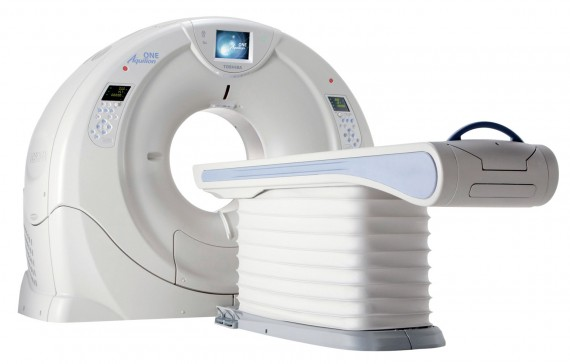
\includegraphics[scale=0.4]{../user_guide_figures/tomografo.jpg}
\caption{Medical CT scanner - www.toshibamedical.com.br}
\end{figure}

Most modern CT scanning appliances are equipped with a radiation emitter and a sensor bank (with channels ranging from 2 to 256), which circle the patient while the stretcher is moved, forming a spiral. This generates a large number of images simultaneously, with little emission of X-rays.

\subsubsection{Hounsfield Scale}

As mentioned in the previous section, the CT images are generated in gray levels, expressed in Hounsfield (HU), wherein lighter shades represent denser matters, and the darker, less dense matter such as skin and brain tissues. 

Table~\ref{tab:escala_hounsfield} presents some materials and their respective values in Hounsfield Units (HU).

\begin{table}[h]
\centering
\caption{Escala de Hounsfield}
\begin{tabular}{lcc}\\
\hline % este comando coloca uma linha na tabela
Material & HU\\
\hline
\hline
Air & -1000 or less\\
Fat & -120\\
Water & 0\\
Muscle & 40\\
Contrast & 130\\
Bone & 400 or more\\
\hline
\end{tabular}
\label{tab:escala_hounsfield}
\end{table}


\subsection{Computed Tomography - Dental (CBCT)}

The dental CT commonly works with less radiation emission compared to medical CT, and therefore makes it possible to view more details of delicate regions such as alveolar cortical.

\begin{figure}[!htb]
\centering
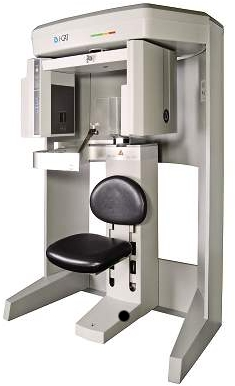
\includegraphics[scale=0.4]{../user_guide_figures/feixe_conico.jpg}
\caption{Dental tomography - www.kavo.com.br}
\end{figure}

Image acquisition is performed with the patient positioned vertically (as opposed to medical tomography in which the patient is horizontal). A transmitter X-ray surround the patient's skull, forming an arc of $180^\circ$ or $360^\circ$. The images generated are compiled as a volume of the patient's skull. This volume is then "sliced" by the software into individual layers, being able to generate images with different spacing or fields of view, such as a panoramic view of the region of interest.

The images acquired by dental scanners often require more post processing when it is necessary to separate (segmental) certain structures using other software such as InVesalius. This is because, typically, these images have more gray levels than, which makes use of segmentation patterns (preset) less. Another very common feature in the images of provincial dental CT scanners is the high presence of speckle noise and other forms of noise typically caused by the presence of amalgam prosthetics.

\subsection{Magnetic Resonance Imaging - MRI}

MRI is an examination performed without the use of ionizing radiation. Instead, it use a strong magnetic field to align the atoms of any element present in our body, most commonly hydrogen. After alignment, radio waves are triggered to excite atoms. The sensors measure the time that the hydrogen atoms take to realign. This makes it possible to distinguish between different tissues, as different types possess different quantities of hydrogen atoms.

To avoid interference and improve the quality of the radiofrequency signal, the patient is placed inside a narrow tube encompassed by the coil and scanning unit.

\begin{figure}[!htb]
\centering
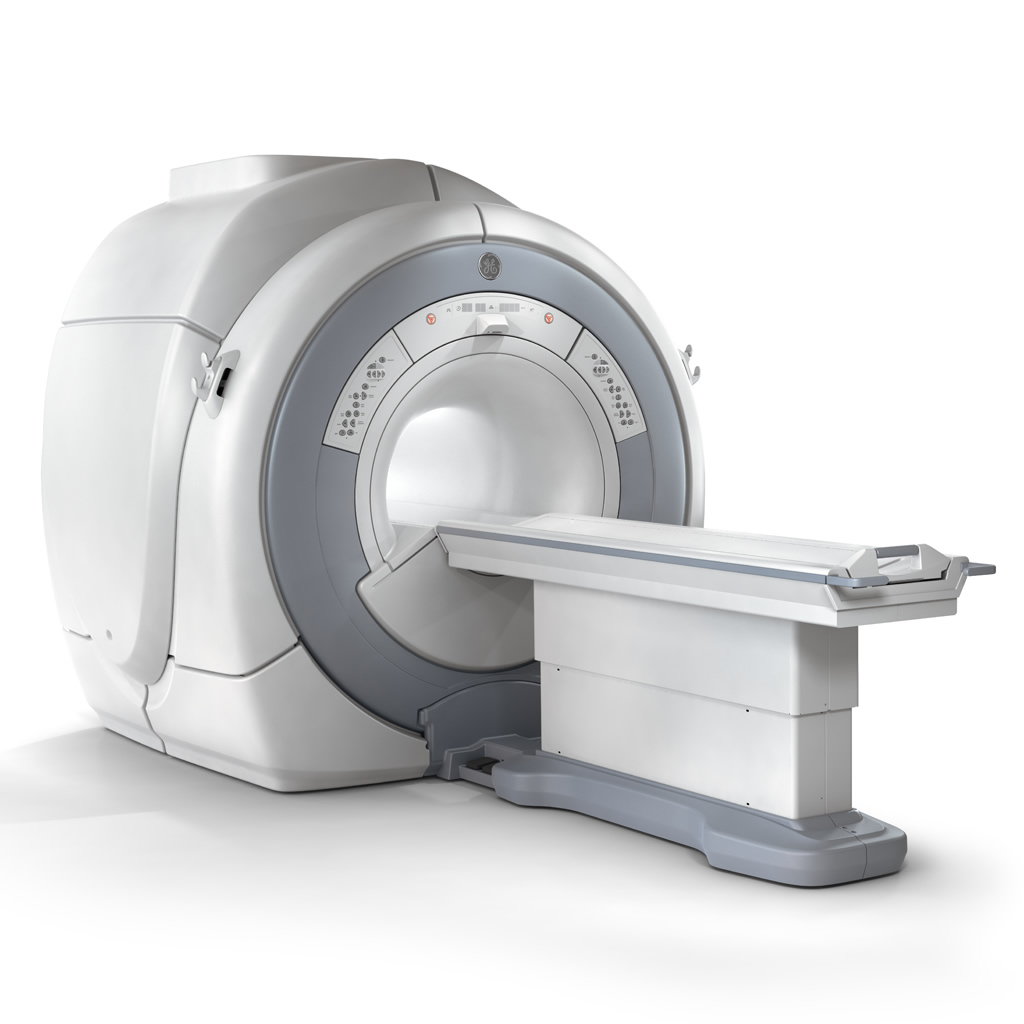
\includegraphics[scale=0.2]{../user_guide_figures/rm_ge.jpg}
\caption{Magnetic resonance imaging equipment - www.gehealthcare.com}
\end{figure}

\begin{figure}[!htb]
\centering
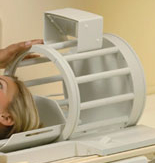
\includegraphics[scale=0.8]{../user_guide_figures/bobina.jpg}
\caption{Coil - www.healthcare.philips.com}
\end{figure}

\subsection{Neuronavigation}
\label{sec:neuronavegador_intro}

Neuronavigation is a technique that allows tracking and localization of surgical instruments relative to neuronal
structures through computer visualization. In addition, neuronavigation systems a fundamental tool to aid surgical plan and to increase the accuracy of experiments in neuroscience, such as transcranial magnetic stimulation (TMS), electroencephalography (EEG), magnetoencephalography (MEG) and near-infrared spectroscopy (NIRS).
Despite the vast field of applications, the use of neuronavigation in research centers is limited by its high cost.
InVesalius Navigator offers users a low-cost, open-source alternative to commercial neuronavigation systems. In this sense, it is possible to use specific tools for
neuronavigation and still have the possibility of developing features on demand. The software for neuronavigation is distributed in an executable version compatible with Windows 7, 8 and 10 operating system. The chapter~\ref{sec:neuronavegador} goes into details of all features of neuronavigation in InVesalius.

\section{Resources needed}

InVesalius is designed to run on personal computers, such as desktops and notebooks. Currently, it is compatible with the following operating systems:

\begin{itemize}
	\item Microsoft Windows (Windows 7, 8, 10)
	\item GNU/Linux (Ubuntu, Mandriva, Fedora) 
	\item Apple Mac OS X
\end{itemize}

The performance of InVesalius depends mainly on the amount of reconstructed slices (images offered by the software), the amount of random access memory (RAM) available, the processor clock rate \& frequency, and operating system architecture (32-bit or 64-bit).

It is important to note that, as a general rule, the greater the amount of RAM available on the system, the greater the number of slices that can be opened simultaneously. For example, with 1 GB of available memory, it can open about 300 slices with a resolution of 512x512 pixels. With 4 GB of memory, around 1000 images can be opened simultaneously at the same resolution.

\subsection{Minimum settings}

\begin{itemize}
	\item 32-bit Operating System
	\item Intel Pentium 4 or equivalent 1.5 GHz
	\item 1 GB of RAM
	\item 10 GB available hard disk space
	\item Graphics card with 64 MB memory
	\item Video resolution of 1024x768 pixels
\end{itemize}


\subsection{Recommended settings}
\begin{itemize}
	\item 64-bit Operating System
	\item Intel Core 2 Duo processor or equivalent 2.5 GHz
	\item 8 GB of RAM
	\item 20 GB available hard disk space
	\item NVidia or ATI graphics card with 128 MB of memory
	\item Video resolution of 1920x1080 pixels
\end{itemize}



\chapter{Installation}

\section{MS-Windows}


To install InVesalius on MS-Windows, simply run the installer program. When a window asking you to confirm the file execution appears, click \textbf{Yes}.

\begin{figure}[!htb]
\centering
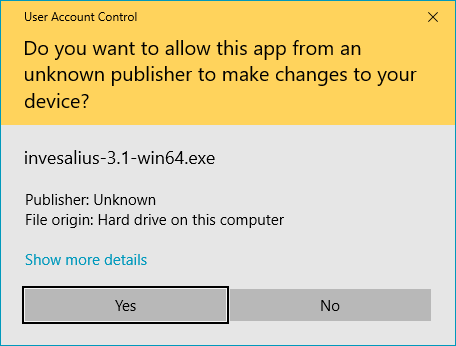
\includegraphics[scale=0.5]{installation_exec_en.png}
\end{figure}

\newpage

A new window will ask you to select the language of the installer. Select the language and click \textbf{OK} button.

\begin{figure}[!htb]
\centering
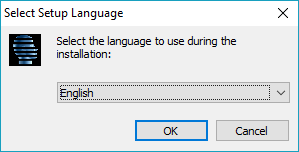
\includegraphics[scale=0.7]{installation_select_language_en.png}
\end{figure}
 
\hspace{.2cm}

Window installer appears. Click \textbf{Next}.


\begin{figure}[!htb]
\centering
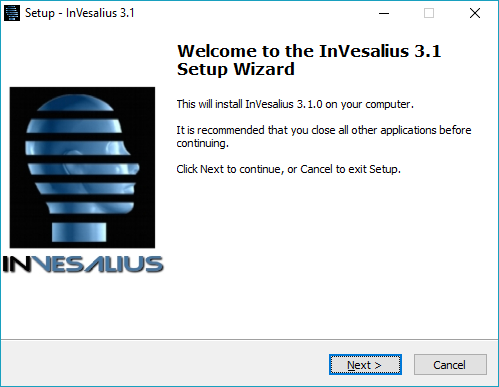
\includegraphics[scale=0.7]{installation_welcome_en.png}
\end{figure}

\newpage

Select \textbf{I accept the agreement} and click on \textbf{Next} button.

\begin{figure}[!htb] 
\centering
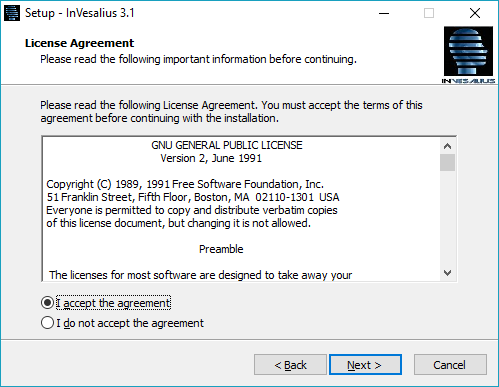
\includegraphics[scale=0.7]{installation_license_en.png}
\end{figure}

\hspace{.2cm}

Click on \textbf{Next} button again. 

\begin{figure}[!htb]  
\centering
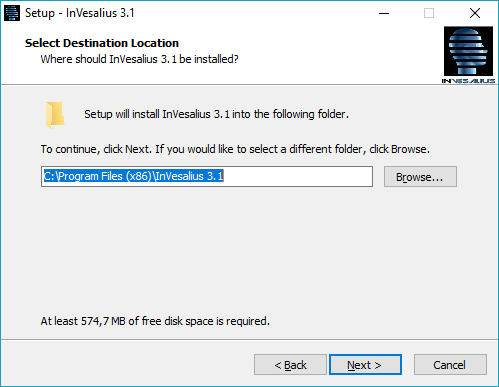
\includegraphics[scale=0.7]{installation_folder_en.png}
\end{figure}

\newpage

Click on \textbf{Next}  button.
\begin{figure}[!htb]
\centering
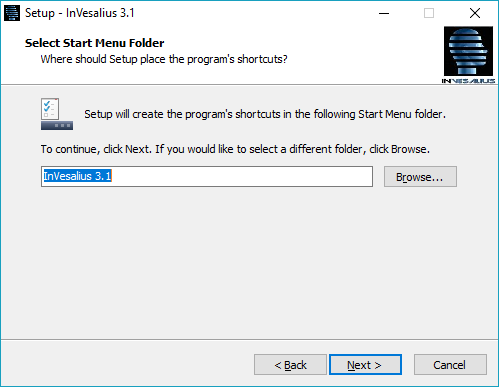
\includegraphics[scale=0.7]{installation_program_name_en.png}
\end{figure}

\hspace{.2cm}

Select \textbf{Create a desktop shortchut} and click on \textbf{Next}.

\begin{figure}[!htb]
\centering
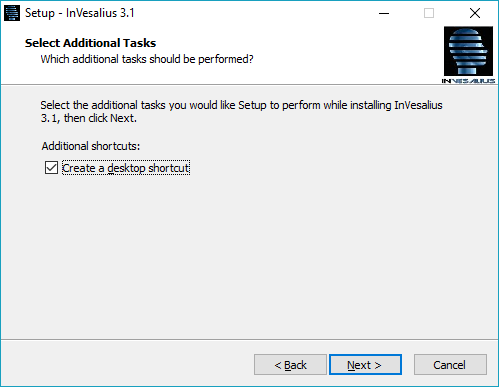
\includegraphics[scale=0.7]{installation_desktop_shortcut_en.png}
\end{figure}

\newpage

Click on \textbf{Install} button.

\begin{figure}[!htb]
\centering
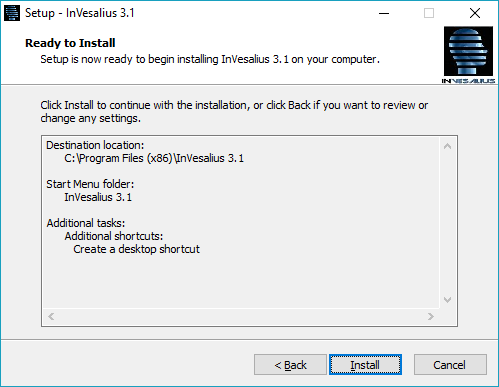
\includegraphics[scale=0.7]{installation_resume_en.png}
\end{figure}

\hspace{.2cm}

While the software is installed, a progress window will appear.

\begin{figure}[!htb]
\centering
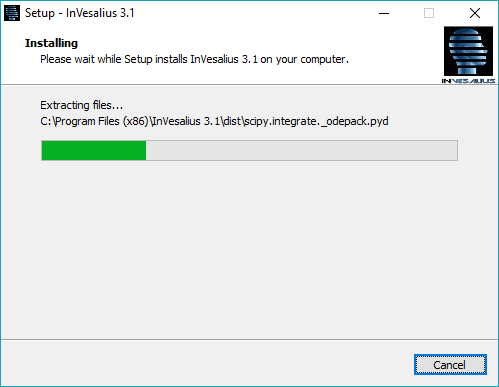
\includegraphics[scale=0.7]{installation_progress_en.png}
\end{figure}

\newpage

To run InVesalius after installation, check \textbf{Lauch InVesalius 3.1} and click on \textbf{Finish} button.

\begin{figure}[!htb]
\centering
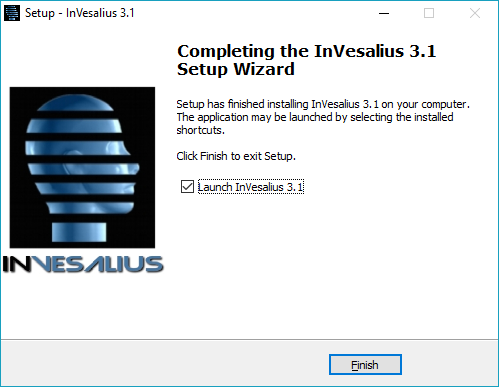
\includegraphics[scale=0.7]{installation_finish_en.png}
\end{figure}

\hspace{.2cm}

If this is the first time the software is installed, a window will appear to select the InVesalius language. Select the language you want and click on \textbf{OK} button.

\begin{figure}[!htb]
\centering
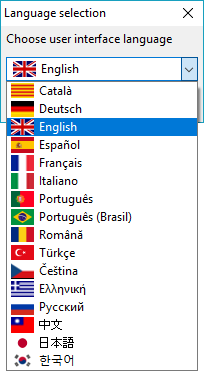
\includegraphics[scale=0.6]{invesalius_language_select_en.png}
\end{figure}

\newpage

While InVesalius is loaded, an opening window like the one in the next figure is displayed.

\begin{figure}[!htb]
\centering
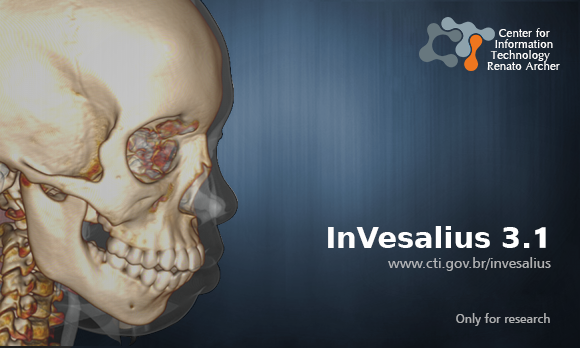
\includegraphics[scale=0.4]{splash_en.png}
\end{figure}

\hspace{.2cm}

Then, the main program window open.

\begin{figure}[!htb]
\centering
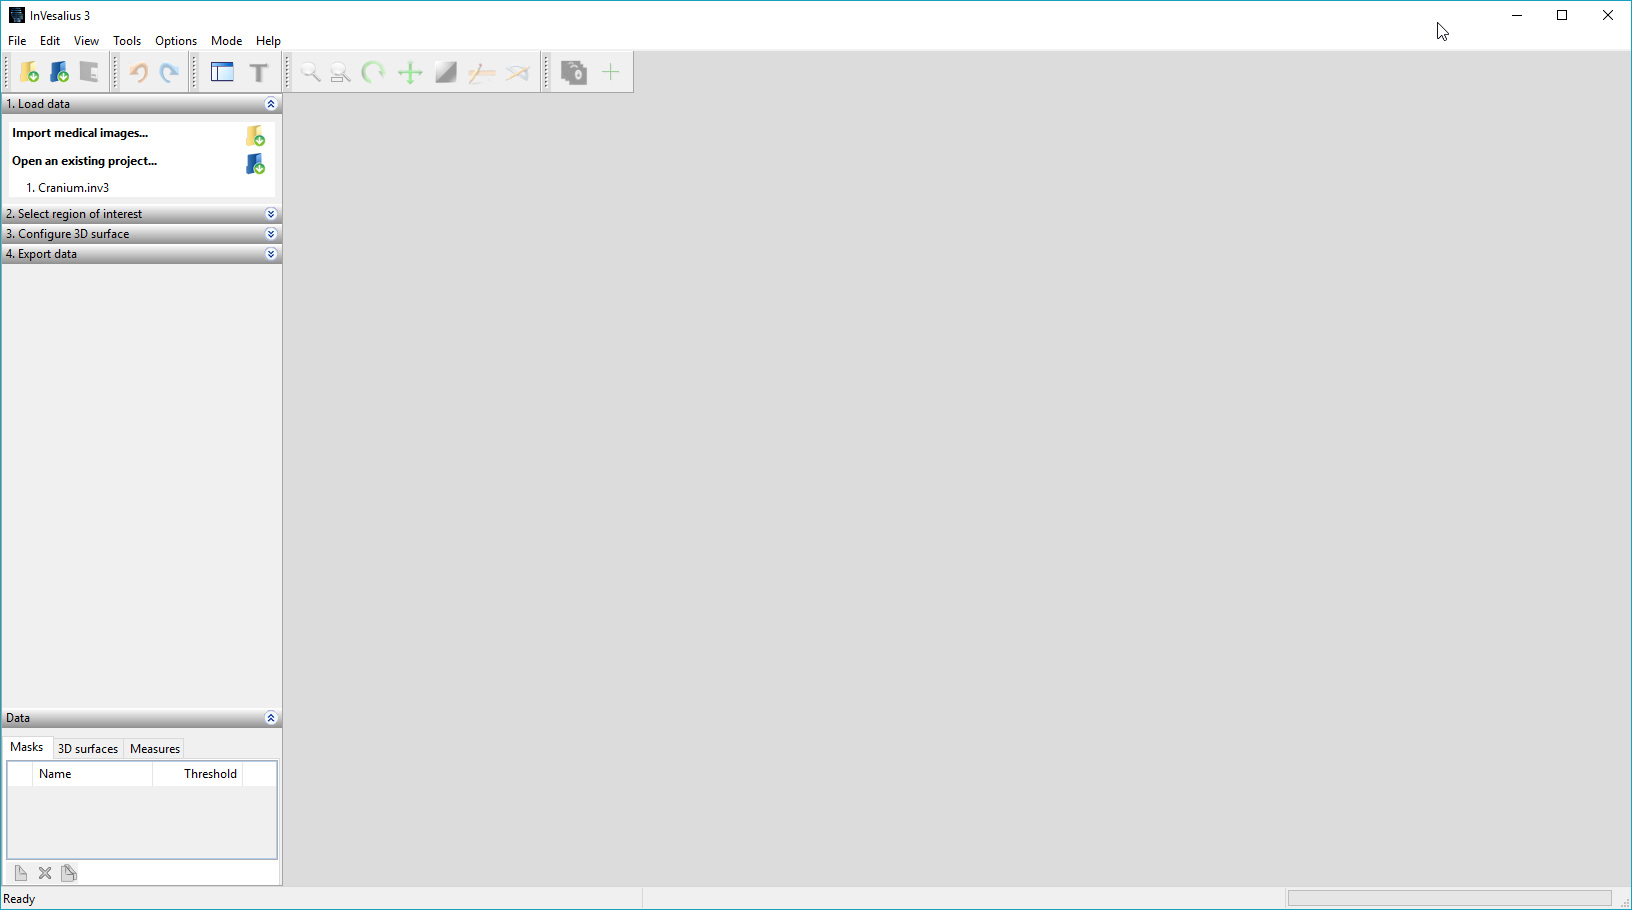
\includegraphics[scale=0.3]{main_window_without_project_en.png}
\end{figure}

\section{Mac Os X}

To start the installation on Mac Os X, double-click the installer with the left mouse button.
Then the installer will be initialized.

\begin{figure}[!htb]
\centering
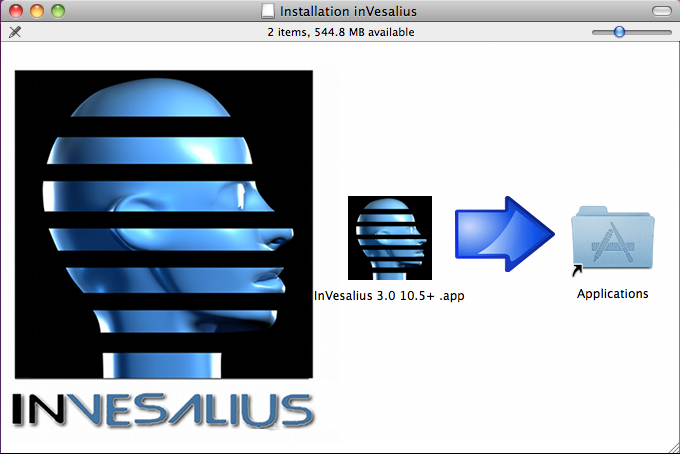
\includegraphics[scale=0.3]{mac2.png}
\end{figure}

Hold down the left button on the InVesalius software icon and drag it to the \textit{Applications}. Both contained in the installer.

\begin{figure}[!htb]
\centering
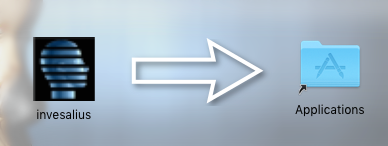
\includegraphics[scale=0.4]{mac4.png}
\end{figure}

The software is already installed, just access through the menu.
\chapter{Image import}

InVesalius imports files in DICOM format, including compressed files (lossless JPEG), Analyze (Mayo Clinic$^\copyright$), NIfTI, PAR/REC, BMP, TIFF, JPEG and PNG formats.

\section{DICOM}

Under the File menu, click on Import DICOM or use the shortcut Ctrl+I. Additionally, DICOM files can be imported by clicking on the icon shown in Figure~\ref{fig:import}.

\begin{figure}[!htb]
\centering

\includegraphics[scale=0.2]{../user_guide_figures/icons/file_import_original.png}
\caption{Shortcut to DICOM import}
\label{fig:import}
\end{figure}

\hspace{.2cm}

Select the directory containing the DICOM files, as in Figure~\ref{fig:win_folder}. InVesalius will search for files also in subdirectories of the chosen directory,
if they exist.

\newpage

Once the directory is selected, click \textbf{OK}.

\begin{figure}[!htb]
\centering
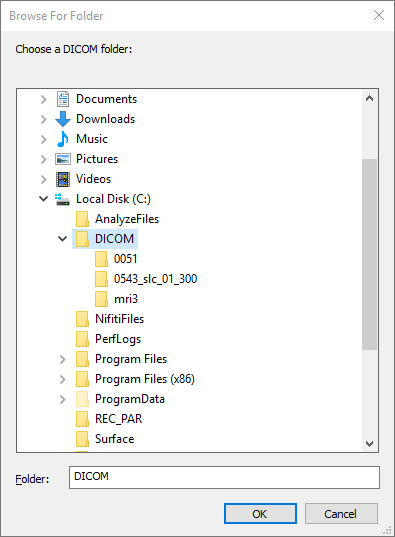
\includegraphics[scale=0.5]{../user_guide_figures/invesalius_screen/import_select_folder_en.png}
\caption{Folder Selection}
\label{fig:win_folder}
\end{figure}

\hspace{.2cm}

While InVesalius search for DICOM files in the directory, the loading progress of the scanned files is displayed, as shown in the Figure~\ref{fig:ver_file}.

\begin{figure}[!htb]
\centering
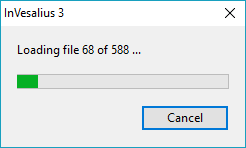
\includegraphics[scale=0.6]{../user_guide_figures/invesalius_screen/import_load_files_en.png}
\caption{Loading file status}
\label{fig:ver_file}
\end{figure}

\newpage

If DICOM files are found, a window open (shown Figure~\ref{fig:win_import}) will open to select the patient and respective series to be opened. It is also possible to skip images for reconstruction.

\begin{figure}[!htb]
\centering
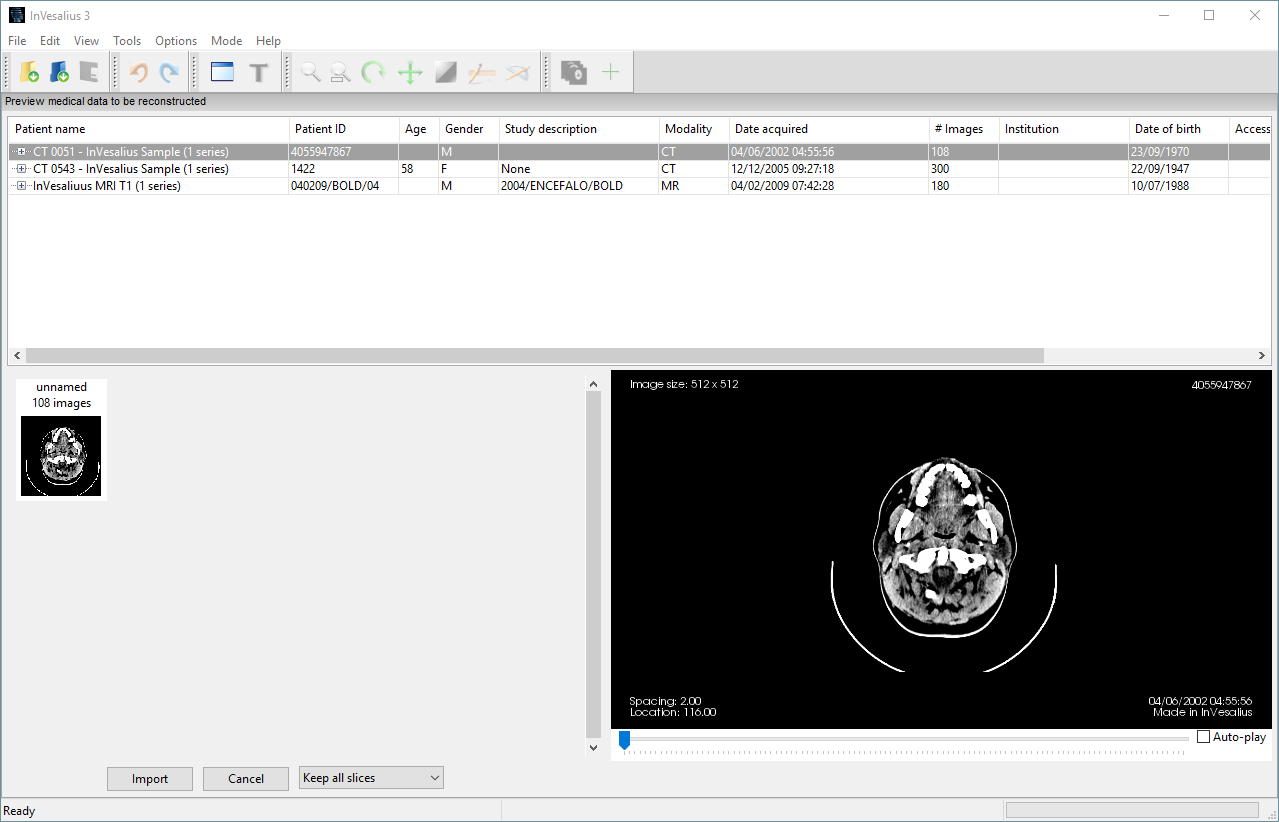
\includegraphics[scale=0.4]{../user_guide_figures/invesalius_screen/import_window_en.png}
\caption{Import window}
\label{fig:win_import}
\end{figure}

\newpage

To import a series with all images present, click "\textbf{$+$}" on the patient’s name to expand the corresponding series. Double-click on the description of the series. See Figure~\ref{fig:import_serie}.

\begin{figure}[!htb]
\centering
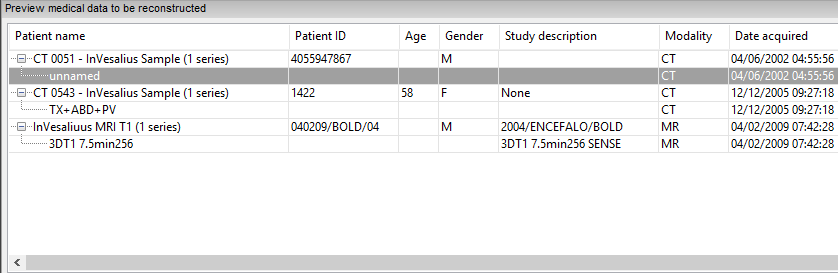
\includegraphics[scale=0.5]{../user_guide_figures/invesalius_screen/import_window_detail_en.png}
\caption{Series selection}
\label{fig:import_serie}
\end{figure}

In some cases, when there is no computer with memory and/or satisfactory processing to work with large numbers of images in a series, it is recommended to skip some of them. To do this, click \textbf{once} with the \textbf{left} mouse button over the description of the series (Figure~\ref{fig:import_serie}) and select how many images will be skipped (Figure~\ref{fig:skip_image}), then click \textbf{Import}.

\begin{figure}[!htb]
\centering
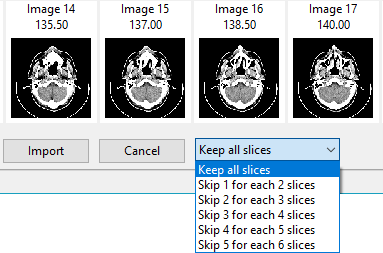
\includegraphics[scale=0.6]{../user_guide_figures/invesalius_screen/import_window_skip_slice_en.png}
\caption{Skip imagens option}
\label{fig:skip_image}
\end{figure}

If there is an insufficient amount of available memory at the time of loading the images it is recommended that the resolution of the slices be reduced to work with volumetric and surface visualization, as shown in Figure~\ref{fig:resize_image}.
The slices will be resized according to the percentage relative to the original resolution. For example, if each slice of the exam the dimension of 512 x 512 pixels and the "Percentage of original resolution" is suggested to be 60 \%, each resulting image will be 307 x 307 pixels. To open with the original pixel resolution, set the percentage to 100.

\begin{figure}[!htb]
\centering
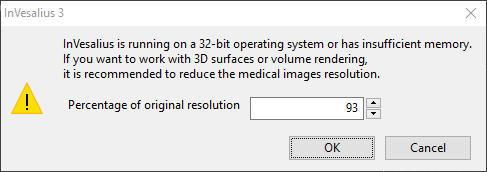
\includegraphics[scale=0.5]{../user_guide_figures/invesalius_screen/import_window_lower_memory_en.png}
\caption{Image size reduction}
\label{fig:resize_image}
\end{figure}

If the image was obtained with the gantry tilted it will be necessary to correct to avoid distortion of any reconstruction. InVesalius allows the user to do this easily. When importing an image with the gantry tilted a dialog will appear, showing the gantry tilt angle. (Figure~\ref{fig:gantry_tilt}). It is possible to change this value, but it is not recommended. Click on the \textbf{Ok} to do the correction. If you click on the \textbf{cancel} button the correction will not be done.

\begin{figure}[!htb]
\centering
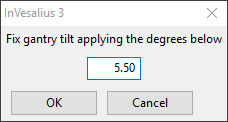
\includegraphics[scale=0.75]{../user_guide_figures/invesalius_screen/window_gantry_tilt_en.png}
\caption{Gantry tilt correction}
\label{fig:gantry_tilt}
\end{figure}

After the above procedure, a window will be displayed (Figure \ref{fig:prog_recons}) with reconstruction (when images are stacked and interpolated).

\begin{figure}[!htb]
\centering
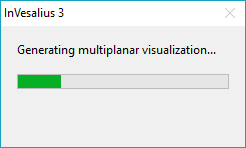
\includegraphics[scale=0.6]{../user_guide_figures/invesalius_screen/import_window_progress_en.png} 
\caption{Reconstruction progress}
\label{fig:prog_recons}
\end{figure}

\newpage

\section{Analyze}

To import Analyze files, under the \textbf{File} menu, click \textbf{Import other files}, then click in the \textbf{Analyze} option as show the Figure~\ref{fig:analyze_menu}.

\begin{figure}[!htb]
\centering
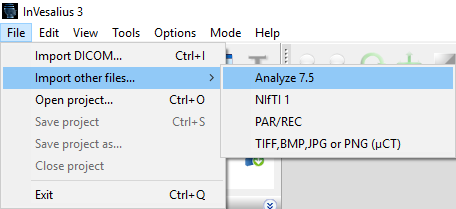
\includegraphics[scale=0.4]{../user_guide_figures/invesalius_screen/import_analyze_menu_en.png}
\caption{Menu for importing images in analyze format.}
\label{fig:analyze_menu}
\end{figure}

Select the Analyze file format (\textbf{.hdr}) and click on \textbf{Open} (Figure~\ref{fig:analyze_import}).
 
\begin{figure}[!htb]
\centering
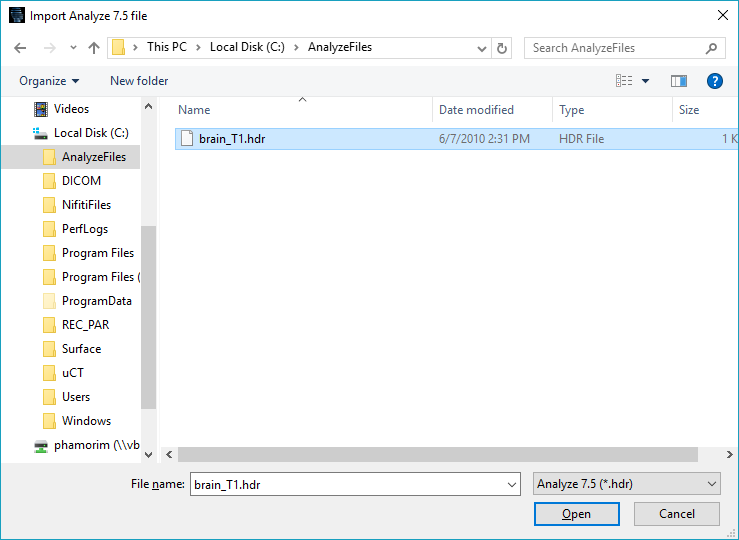
\includegraphics[scale=0.4]{../user_guide_figures/invesalius_screen/import_analyze_window_en.png}
\caption{Import analyze file format}
\label{fig:analyze_import}
\end{figure}

\section{NIfTI}

To import NIfTI files, under the \textbf{File}  menu, click \textbf{Import other files} and then click \textbf{NIfTI} as shown in Figure~\ref{fig:import_nifti_menu_pt}.


\begin{figure}[!htb]
\centering
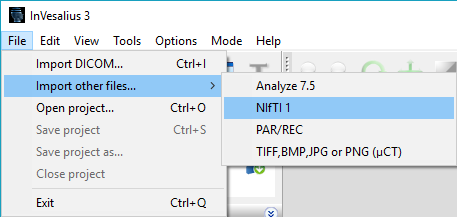
\includegraphics[scale=0.4]{../user_guide_figures/invesalius_screen/import_nifti_menu_en.png}
\caption{Menu to import images in NIfTI format}
\label{fig:import_nifti_menu_pt}
\end{figure}

Select the NIfTI file format, (either \textbf{nii.gz} or \textbf{.nii}) then click \textbf{Open} (Figure~\ref{fig:import_nifti_window_pt}). If the file is in another format as \textbf{.hdr}, select \textbf{all files(*.*)} option.

\begin{figure}[!htb]
\centering
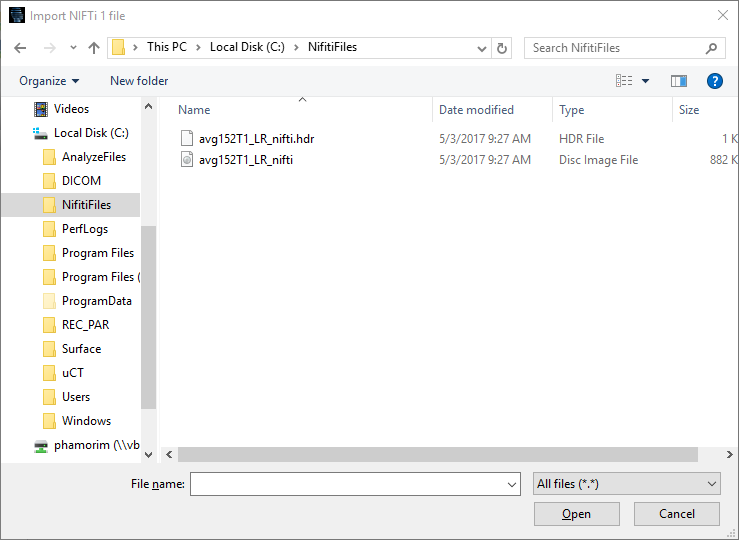
\includegraphics[scale=0.4]{../user_guide_figures/invesalius_screen/import_nifti_window_en.png}
\caption{Importing images in NIfTI format.}
\label{fig:import_nifti_window_pt}
\end{figure}

\section{PAR/REC}

To import PAR/REC file, under the \textbf{File} menu, click \textbf{Import other files}, and then click on \textbf{PAR/REC} as shown in Figure~\ref{fig:import_parrec_menu_pt}.

\begin{figure}[!htb]
\centering
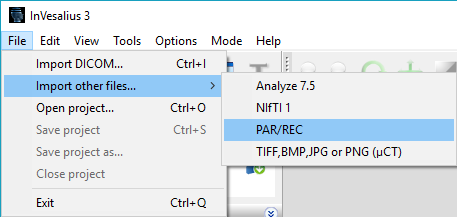
\includegraphics[scale=0.4]{../user_guide_figures/invesalius_screen/import_parrec_menu_en.png}
\caption{Menu for importing PAR/REC images}
\label{fig:import_parrec_menu_pt}
\end{figure}

Select PAR/REC file type, with the file extension \textbf{.par} and click \textbf{Open} (Figure~\ref{fig:import_parrec_window_pt}). If the file has no extension, select \textbf{all files(*.*)} option.

\begin{figure}[!htb]
\centering
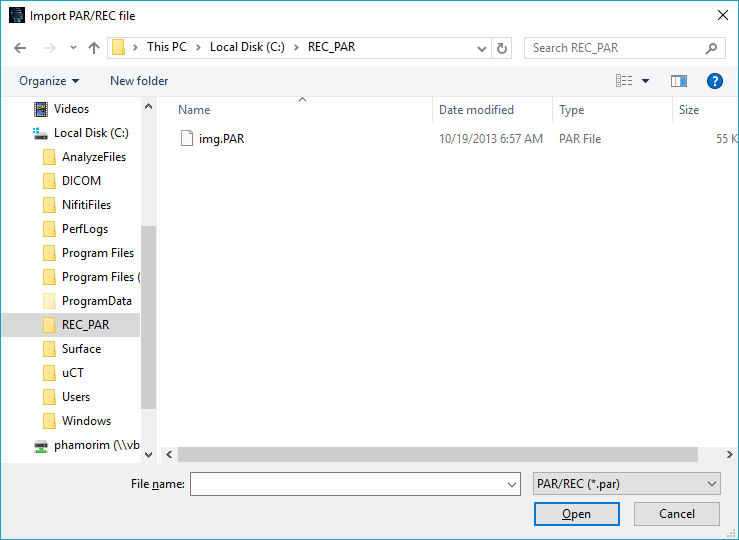
\includegraphics[scale=0.4]{../user_guide_figures/invesalius_screen/import_parrec_window_en.png}
\caption{PAR/REC import}
\label{fig:import_parrec_window_pt}
\end{figure}

\section{TIFF, JPG, BMP, JPEG or PNG (micro-CT)}

TIFF, JPG, BMP, JPEG or PNG file format for microtomography equipment (micro-CT or $\mu$CT) or others. InVesalius imports files in these formats if pixels present are represented in \textbf{grayscale}.

To import, click on menu \textbf{File}, \textbf{Import other files...} and then click on \textbf{TIFF, JPG, BMP, JPEG ou PNG ($\mu$CT)} option as shown the figure~\ref{fig:import_bmp_menu_pt}.

\begin{figure}[!htb]
\centering
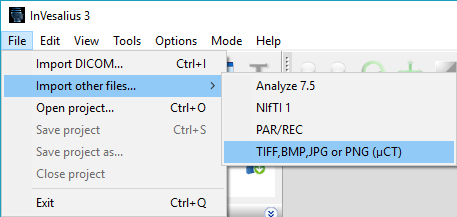
\includegraphics[scale=0.4]{../user_guide_figures/invesalius_screen/import_bmp_menu_en.png}
\caption{Import images in BMP and others formats}
\label{fig:import_bmp_menu_pt}
\end{figure}

Select the directory that contains the files, as shown the Figure~\ref{fig:import_bmp_select_folder}. InVesalius will search for files also in subdirectories of the chosen directory, if they exist. 

Click on \textbf{OK}.

\begin{figure}[!htb]
\centering
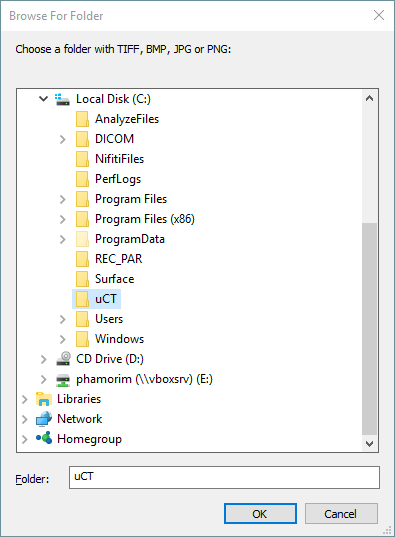
\includegraphics[scale=0.5]{../user_guide_figures/invesalius_screen/import_bmp_select_folder_en.png}
\caption{Folder selection}
\label{fig:import_bmp_select_folder}
\end{figure}

While InVesalius is looking for TIFF, JPG, BMP, JPEG, or PNG files in the directory, the upload progress of the scanned files is displayed, as illustrated in Figure~\ref{fig:import_bmp_load_pt}.

\begin{figure}[!htb]
\centering
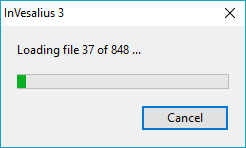
\includegraphics[scale=0.6]{../user_guide_figures/invesalius_screen/import_bmp_load_en.png}
\caption{Checking and loading files status.}
\label{fig:import_bmp_load_pt}
\end{figure}

If files in the desired formats are located, a window will open (shown in Figure~\ref{fig:import_bmp_window_pt}) to display the files eligible for reconstruction. Images can also be skipped to remove files from the rebuild list. The files are sorted according to file names. It is recommended that the files are numbered according to the desired rebuild order.

\begin{figure}[!htb]
\centering
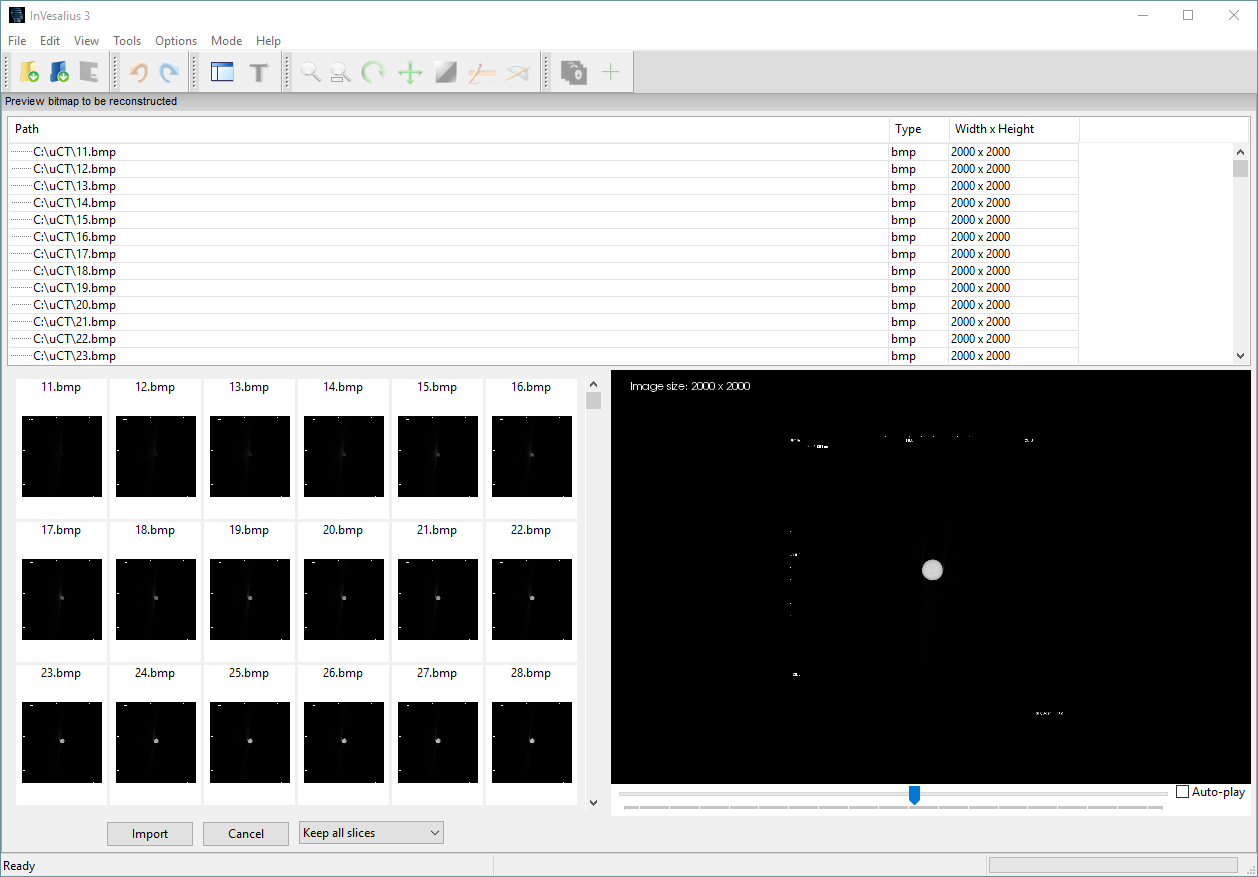
\includegraphics[scale=0.3]{../user_guide_figures/invesalius_screen/import_bmp_window_en.png}
\caption{Window to import BMP files.}
\label{fig:import_bmp_window_pt}
\end{figure}
 
To delete files that are not of interest, select a file by clicking the left mouse button and then pressing the delete key. You can also choose a
range of files to delete by clicking the \textbf{left mouse button} on a file, holding down the \textbf{shift} key, clicking again with the mouse button in the last file of the track and finally pressing the \textbf{delete} button.

Similar to when importing DICOM files, you can skip BMP images for re-building. In some cases, particularly where a computer with satisfactory memory and/or processing is unavailable, it may be advisable to skip some of them to retain adequate program functionality. To do this, select how many images to skip (Figure~\ref{fig:import_bmp_skip_pt}), then click \textbf{Import}.

\begin{figure}[!htb]
\centering
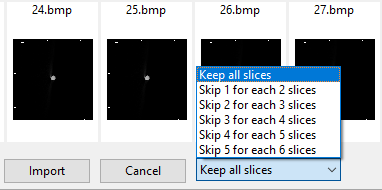
\includegraphics[scale=0.4]{../user_guide_figures/invesalius_screen/import_bmp_skip_en.png}
\caption{Importation window}
\label{fig:import_bmp_skip_pt}
\end{figure}

To reconstruct files of this type, a project name must be defined to indicate the orientation of the images (axial, coronal or sagittal), voxel spacing ($X$, $Y$ and $Z$) in \textbf{mm} as shown in the Figure~\ref{fig:import_bmp_spacing_pt}. The voxel spacing in $X$ is the pixel width of each image, $Y$ the pixel length, and $Z$ represents the distance of each slice (voxel height).

If the image set consists of microtomography images, more specifically GE and Brucker equipment, it is possible that InVesalius will read the text file with the acquisition parameters that normally stay in the same folder as the images and automatically insert the spacing. This verification can be done when the values of $X$, $Y$ and $Z$ are different from "1.00000000", otherwise it is necessary to enter the values of the respective spacing.

\textbf{Correct spacing is crucial for correctly importing objects in InVesalius. Incorrect spacing will provide incorrect measurements.}

Once all parameters have been input, click \textbf{OK}.

\begin{figure}[!htb]
\centering
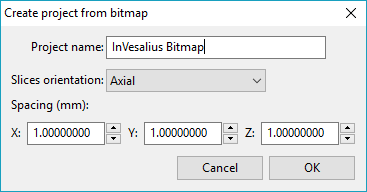
\includegraphics[scale=0.5]{../user_guide_figures/invesalius_screen/import_bmp_spacing_en.png}
\caption{Import Screen}
\label{fig:import_bmp_spacing_pt}
\end{figure}

If insufficient memory is available when loading images, it is recommended to reduce the resolution of the slices to work with volumetric and surface visualization, as shown in Figure~\ref{fig:import_bmp_resize_pt} window.The slices will be resized according to the percentage relative to the original resolution. For example, if each slice of the exam contains the dimension of $512 x 512$ pixels and the "Percentage of the original resolution" is suggested at 60, each resulting image will have $307 x 307$ pixels. If you want to open with the original resolution set the percentage to $100$.

\begin{figure}[!htb]
\centering
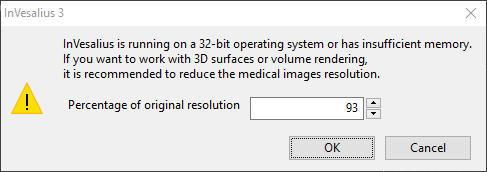
\includegraphics[scale=0.5]{../user_guide_figures/invesalius_screen/import_window_lower_memory_en.png}
\caption{Image resize}
\label{fig:import_bmp_resize_pt}
\end{figure}

After the previous steps, wait a moment for the program to complete the multiplanar reconstruction as shown in Figure~\ref{fig:import_bmp_mpr_pt.png}.

\begin{figure}[!htb]
\centering
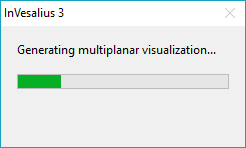
\includegraphics[scale=0.6]{../user_guide_figures/invesalius_screen/import_window_progress_en.png}
\caption{Multiplanar reconstruction in progress.}
\label{fig:import_bmp_mpr_pt.png}
\end{figure}

\chapter{Image adjustment}

InVesalius cannot guarantee the correct image order; images may contain incorrect information, or do not follow the DICOM standard. Therefore, it is recommended to check if a lesion or an anatomical mark is on the correct side. If not, it is possible to use the flip image or swap axes tools. For image alignment, the rotation image tool can be used.

It is possible to mirror the image. To do so, select the \textbf{Tools} menu, click \textbf{Image}, then \textbf{Flip} and click on one of the following options (Figure~\ref{fig:menu_img_mirroring_axis_pt}):

\begin{itemize}
	\item Right - Left
	\item Anterior - Posterior
	\item Top - Botton
\end{itemize}

\begin{figure}[!htb]
\centering
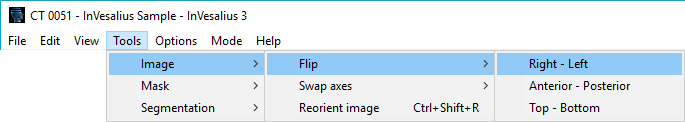
\includegraphics[scale=0.4]{menu_img_mirroring_axis_en.png}
\caption{Menu to activate flip image tool.}
\label{fig:menu_img_mirroring_axis_pt}
\end{figure}


Figure~\ref{fig:mirrored} shows a comparison between the input image and the flipped image. All other orientations are also modified when the image is flipped.

\begin{figure}[!htb]
  \centering
  \subfloat[Input image]{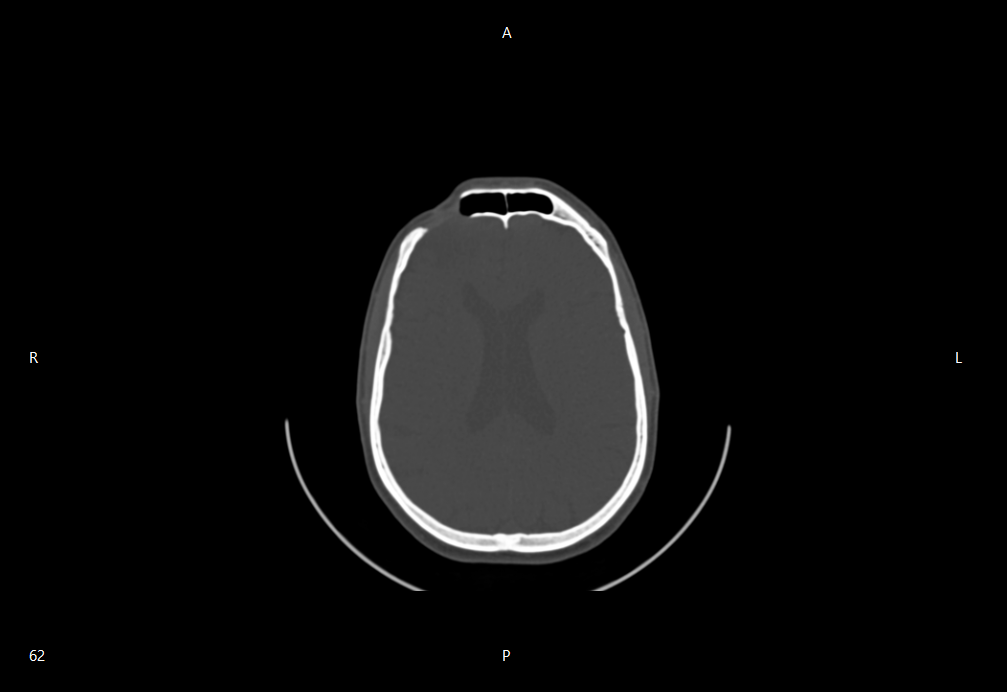
\includegraphics[width=0.45\textwidth]{mirror_axial_en.png}}  \qquad
  \subfloat[Flipped image]{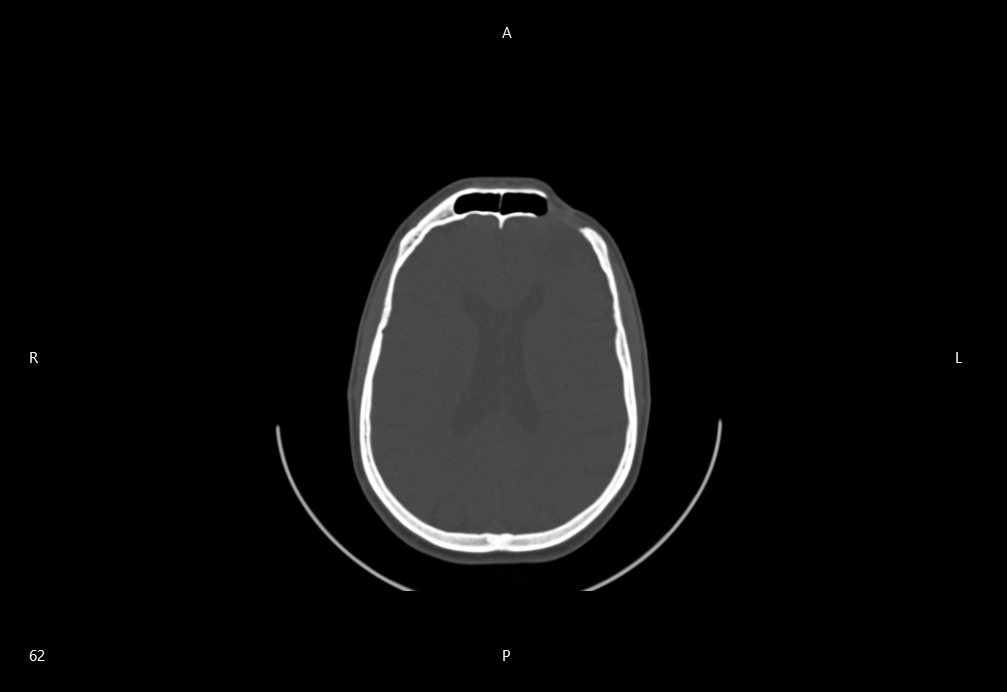
\includegraphics[width=0.45\textwidth]{mirror_axial_mirrored_en.png}}
  \hfill
  \caption{Example of a right-left flipped image.}
  \label{fig:mirrored}
\end{figure}

\section{Swap axes}

The swap axes tool changes the image orientation, in the case that the image has been wrongly imported. To perform this, select the \textbf{Tools} menu, click \textbf{Image}, then \textbf{Swap Axes} and click on one of the following options (Figure~\ref{fig:menu_invert_axis}):

\begin{itemize}
	\item From Right-Left to Anterior-Posterior
	\item From Right-Left to Top-Bottom
	\item From Anterior-Posterior to Top-Bottom
\end{itemize}


The Figures~\ref{fig:invert_axis_axial} and~\ref{fig:invert_axis_axial_inverted}, shows an example of an image with inverted axes.

\begin{figure}[!htb]
\centering
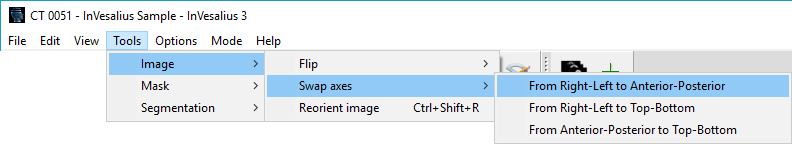
\includegraphics[scale=0.4]{menu_invert_axis_en.png}
\caption{Menu to activate swap image tool.}
\label{fig:menu_invert_axis}
\end{figure}

\begin{figure}[!htb]
\centering
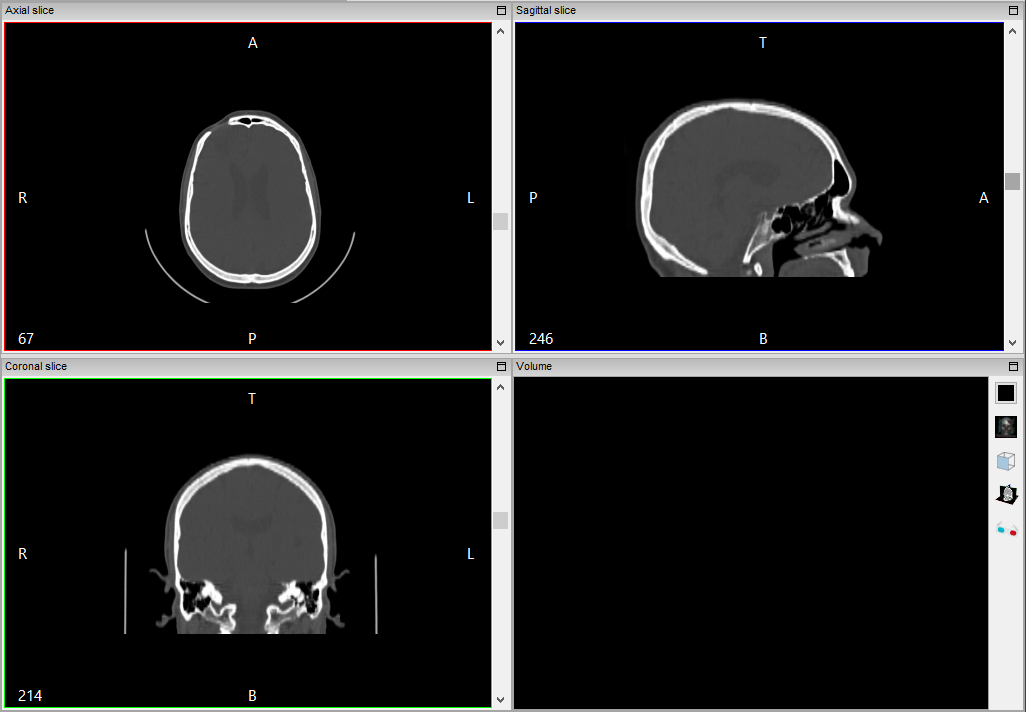
\includegraphics[scale=0.4]{invert_axis_axial_en.png}
\caption{Images before swap axes - from Anterior-Posterior to Top-Bottom.}
\label{fig:invert_axis_axial}
\end{figure}

\begin{figure}[!htb]
\centering
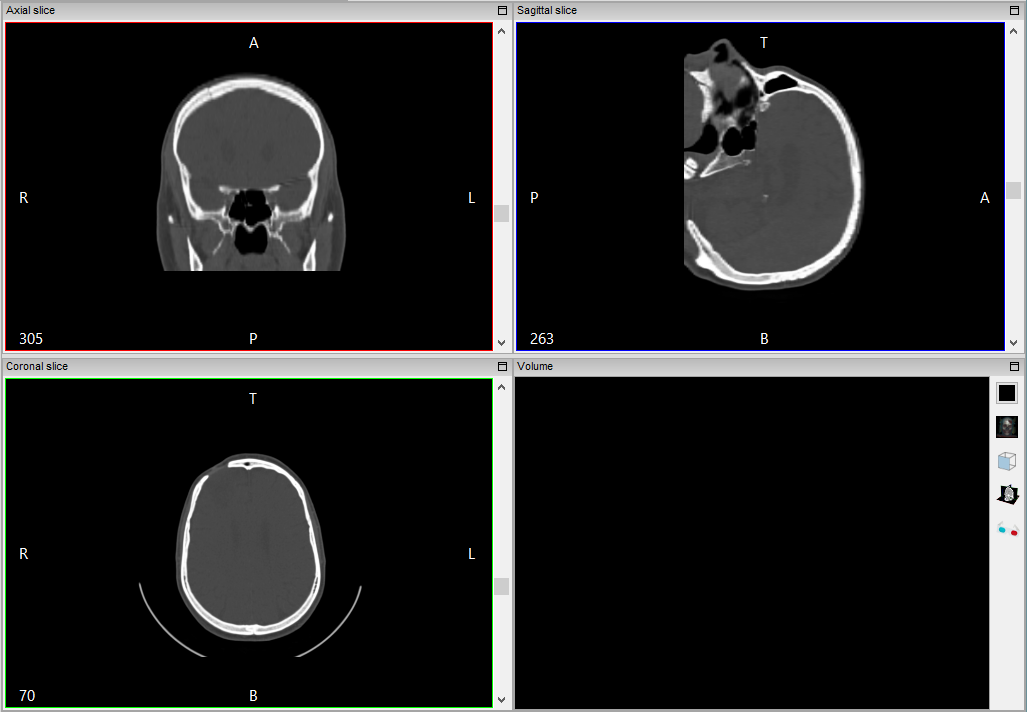
\includegraphics[scale=0.4]{invert_axis_axial_inverted_en.png}
\caption{Images after swap axes - from Anterior-Posterior to Top-Bottom.}
\label{fig:invert_axis_axial_inverted}
\end{figure}

\section{Reorient image (Rotate)}

If it is necessary to align the image with a certain point of reference, e.g. anatomical marker, use the reorient image tool. To open this tool select the \textbf{Tools} menu, click \textbf{Image}, then \textbf{Reorient Image} (Figure~\ref{fig:menu_img_reorient}).

\begin{figure}[!htb]
\centering
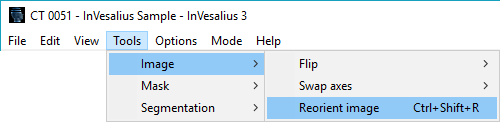
\includegraphics[scale=0.4]{menu_img_reorient_en.png}
\caption{Menu to activate reorient image tool.}
\label{fig:menu_img_reorient}
\end{figure}

When this tool is activated a window is opened (Figure~\ref{fig:image_reorient_window}) showing orientation and by how many degrees the image was rotated.

\begin{figure}[!htb]
\centering
\includegraphics[scale=0.4]{image_reorient_window_en.png}
\caption{Window that shows the reorientation image parameters.}
\label{fig:image_reorient_window}
\end{figure}

To start reorienting the image, define the rotation point by keeping the \textbf{left} mouse button pressed between the two lines intersecting (Figure~\ref{fig:image_reorient_adjust_center}) at one orientation, e.g. axial, coronal or sagittal, and \textbf{drag} to the desired point.

\begin{figure}[!htb]
\centering
\includegraphics[scale=0.4]{image_reorient_adjust_center_en.png}
\caption{Defining the axis of rotation of the image.}
\label{fig:image_reorient_adjust_center}
\end{figure}

To rotate the image it is necessary to keep the \textbf{left} mouse button pressed and \textbf{drag} until the reference point or anatomical marker stays aligned with one of the lines (Figure~\ref{fig:image_reorient_rotated}). After the image is in the desired position, click \textbf{Apply} in the parameter window (Figure~\ref{fig:image_reorient_window}). This may take a few moments depending on the image size. Figure~\ref{fig:image_reorient_rotated_applied} shows an image successfully reoriented.

\begin{figure}[!htb]
\centering
\includegraphics[scale=0.4]{image_reorient_rotated_en.png}
\caption{Rotated image.}
\label{fig:image_reorient_rotated}
\end{figure}

\begin{figure}[!htb]
\centering
\includegraphics[scale=0.4]{image_reorient_rotated_applied_en.png}
\caption{Rotated image after reorientation is done.}
\label{fig:image_reorient_rotated_applied}
\end{figure}

\chapter{Image Manipulation (2D)}

\section{Multiplanar Reconstruction}

When images are imported, InVesalius automatically shows its multiplanar reconstruction in the Axial, Sagittal and Coronal orientations, as well as a window for 3D manipulation, as seen in Figure~\ref{fig:mpr}.

\begin{figure}[!htb]
\centering
\includegraphics[scale=0.40]{multiplanar_mask_window_en.png}
\caption{Multiplanar Reconstruction}
\label{fig:mpr}
\end{figure}

\newpage

In addition to creating a multiplanar reconstruction, InVesalius segments an image, highlighting for example soft tissue bones. The highlight is represented by the application of colors on a segmented structure so that the colors form a mask over an image highlighting the structure (Figure~\ref{fig:mpr}).This is discussed in more detail in the following chapters.

To hide the mask, use the data manager, located in the lower left corner of the screen. Select the \textbf{Masks} tab and click once using the \textbf{left} mouse button over the eye icon next to \textbf{"Mask 1"}, as shown in Figure~\ref{fig:ger_masc}.

\begin{figure}[!htb]
\centering
\includegraphics[scale=0.8]{data_mask_en.png}
\caption{Mask manager}
\label{fig:ger_masc}
\end{figure}

The eye icon disappears, and the colors of the segmentation mask are hidden (Figure~\ref{fig:mpr_sem_mask}).

\begin{figure}[!htb]
\centering
\includegraphics[scale=0.30]{multiplanar_window_en.png}
\caption{Multiplanar reconstruction without segmentation mask}
\label{fig:mpr_sem_mask}
\end{figure}

\subsection{Axial orientation}

The axial orientation consists of cuts made transversally to the region of interest, i.e. parallel cuts to the axial plane of the human body.
In Figure~\ref{fig:axial_corte}, an axial image of the skull region is displayed.

\begin{figure}[!htb]
\centering
\includegraphics[scale=0.30]{axial_en.png}
\caption{Axial slice}
\label{fig:axial_corte}
\end{figure}

\subsection{Sagittal orientation}

The sagittal orientation consists of cuts made laterally in relation to the region of interest, i.e. parallel cuts to the sagittal plane of the human body, which divides it into the left and right portions.
In Figure~\ref{fig:sagital_slice}, a sagittal skull image is displayed.

\begin{figure}[!htb]
\centering
\includegraphics[scale=0.30]{sagital_en.png}
\caption{Sagittal slice}
\label{fig:sagital_slice}
\end{figure}

\newpage

\subsection{Coronal orientation}

The coronal orientation is composed of cuts parallel to the coronal plane, which divides the human body into ventral and dorsal halves.
In Figure~\ref{fig:coronal_slice} is displayed a skull image in coronal orientation.

\begin{figure}[!htb]
\centering
\includegraphics[scale=0.30]{coronal_en.png}
\caption{Coronal slice}
\label{fig:coronal_slice}
\end{figure}


\section{Correspondence between the axial, sagittal and coronal orientations}
\label{sec:corresp_all_orient}

To find out the common point of intersection of the images in differents orientations, simply activate the "Slices cross intersection" feature with the shortcut icon located on the toolbar. See Figure~\ref{fig:cross_icon}.

\begin{figure}[!htb]
\centering
\includegraphics[scale=1]{cross.png}
\caption{Shortcut to show common point between different orientations}
\label{fig:cross_icon}
\end{figure}

When the feature is activated, two cross-sections that intersect perpendicularly are displayed on each image (Figure~\ref{fig:cross_all}). The intersection point of each pair of segments represents the common point between differents orientations.

\newpage

To modify the point, hold down the \textbf{left} mouse button and \textbf{drag}. Automatically, the corresponding points will be updated in each image.

\begin{figure}[!htb]
\centering
\includegraphics[scale=0.4]{multiplanar_window_cross_en.png}
\caption{Common point between differents orientations}
\label{fig:cross_all}
\end{figure}

To deactivate the feature, simply click on the shortcut again (Figure~\ref{fig:cross_icon}). This feature can be used in conjunction with the slice editor (which will be discussed later).

\section{Interpolation}

By default the 2D images visualization are interpolated (Figure~\ref{fig:interp}).a). To deactivate this feature, select the \textbf{View} menu and select \textbf{Interpolated slices} (Figure~\ref{fig:menu_interpoleted_image_pt}). It will then be possible to visualize each pixel individually as shown in Figure~\ref{fig:interp}.b.

\textbf{This interpolation is for visualization purposes only, and does not directly influence segmentation or 3D surface generation.}

\begin{figure}[!htb]
\centering
\includegraphics[scale=0.7]{menu_interpoleted_image_en.png}
\caption{Menu to disable and enable interpolation}
\label{fig:menu_interpoleted_image_pt}
\end{figure}


\begin{figure}[!htb]
  \centering
  \subfloat[Interpolated]{\includegraphics[width=0.4\textwidth]{axial_interpoleted.png}}  \qquad
  \subfloat[Non-interpolated]{\includegraphics[width=0.4\textwidth]{axial_not_interpoleted.png}}
  \hfill
  \caption{Interpolated and non-interpolated image visualization.}
  \label{fig:interp}
\end{figure}

\section{Move}

To move an image on the screen, use the Move shortcut icon on the toolbar (Figure~\ref{fig:move_icon}). Click on the icon to activate, then with the \textbf{left} mouse button on the image, \text{drag} it to the desired direction. Figure~\ref{fig:move_img} shows a displaced (moved) image.

\begin{figure}[!htb]
\centering
\includegraphics[scale=0.25]{tool_translate_original.png}
\caption{Shortcut to move images}
\label{fig:move_icon}
\end{figure}

\begin{figure}[!htb]
\centering
\includegraphics[scale=0.20]{axial_pan_en.png}
\caption{Displaced image}
\label{fig:move_img}
\end{figure}

\section{Rotate}

Images can be rotated by using the Rorate shortcut on the toolbar (Figure~\ref{fig:rot_icon}). To rotate an image, click on the icon and then with the \textbf{left} mouse button \textbf{drag} clockwise or anticlockwise as required.

\begin{figure}[!htb]
\centering
\includegraphics[scale=0.20]{tool_rotate_original.png}
\caption{Shortcut to rotate images}
\label{fig:rot_icon}
\end{figure}

\begin{figure}[!htb]
\centering
\includegraphics[scale=0.20]{axial_rotate_en.png}
\caption{Rotated image}
\label{fig:rotate_all}
\end{figure}


\section{Zoom}

In InVesalius, there are different ways to enlarge an image. You can maximize the desired orientation window, apply zoom directly to the image, or select the region of the image to enlarge. Each of these methods are detailed below.

\subsection{Maximizing orientation windows}

The main InVesalius window is divided into 4 sub-windows: axial, sagittal, coronal and 3D. Each of these can be maximized to occupy the entire area of the main window. To do this, simply \textbf{left} mouse click on the subwindow icon located in the \textbf{upper right corner} (Figure~\ref{fig:maximize_window}). To restore a maximized window to its previous size, simply click the icon again.

\begin{figure}[!htb]
\centering
\includegraphics[scale=0.6]{maximize_sagital_mpr.png}
\caption{Detail of a sub-window (Note the maximize icon in the upper right corner)}
\label{fig:maximize_window}
\end{figure}

\subsection{Enlarging or shrinking an image}

To enlarge or shrink an image, click on the zoom shortcut icon in the toolbar (Figure~\ref{fig:zoom_icon}). Hold down the \textbf{left} mouse button on the image and \textbf{drag} the mouse \textbf{up} to enlarge or \textbf{down} to shrink.

\begin{figure}[!htb]
\centering
\includegraphics[scale=0.25]{tool_zoom_original.png}
\caption{Zoom shortcut}
\label{fig:zoom_icon}
\end{figure}

\subsection{Enlarging an image area}

To enlarging a certain image area, click on the "Zoom based on selection" icon in the toolbar (Figure~\ref{fig:zoom_icon_loc}). Position the mouse pointer at the origin point of the selection, click and hold the \textbf{left} mouse button and \textbf{drag} it to the end selection point to form a rectangle (Figure~\ref{fig:zoom_select}). Once the left mouse button is released, the zoom operation will be applied to the selected region (Figure~\ref{fig:zoom_applied}).

\begin{figure}[!htb]
\centering
\includegraphics[scale=0.25]{tool_zoom_select_original.png}
\caption{Zoom based on selection shortcut}
\label{fig:zoom_icon_loc}
\end{figure}

\begin{figure}[!htb]
\centering
\includegraphics[scale=0.25]{tool_zoom_select_image_en.png}
\caption{Area selected for zoom}
\label{fig:zoom_select}
\end{figure}

\begin{figure}[!htb]
\centering
\includegraphics[scale=0.25]{tool_image_with_zoom_en.png}
\caption{Enlarged Image}
\label{fig:zoom_applied}
\end{figure}


\section{Brightness and contrast (Windows)}
\label{sec:ww_wl}

To improve image visualization, the \textit{window width} and \textit{window level} features can be used; these are more commonly known as \textit{brightness and contrast} or \textit{window} (for radiologists). With this feature, it is possible to set the range of the gray scale (\textit{window level}) and the width of the scale (\textit{window width}) to be used to display the images.

The feature can be activated by the "Brightness and Contrast" shortcut icon in the toolbar. See Figure~\ref{fig:window_level_shortcut}.

\begin{figure}[!htb]
\centering
\includegraphics[scale=0.70]{tool_contrast_original.png}
\caption{Brightness and contrast shortcut}
\label{fig:window_level_shortcut}
\end{figure}

To increase the brightness, hold down the \textbf{left} mouse button and \textbf{drag} horizontally to the right. To decrease the brightness, simply drag the mouse to the left. The contrast can be changed by dragging the mouse (with the \textbf{left} button pressed) vertically: up to increase, or down to decrease contrast.

To deactivate the feature, click again on the shortcut icon (Figure~\ref{fig:window_level_shortcut}).

Preset brightness and contrast patterns may be used with InVesalius. Table~\ref{tab:window_level} lists some tissue types with their respective brightness and contrast values. To use the presets, position the mouse cursor over an image and \textbf{right-click} to open a context menu, then select \textbf{Window width and level}, and click on the preset option according to the tissue type, as shown in Figure~\ref{fig:window_level}.

\begin{figure}[!htb]
\centering
\includegraphics[scale=0.40]{menu_window_and_level_en.png}
\caption{Context menu for brightness and contrast selection}
\label{fig:window_level}
\end{figure}

\begin{table}[!h]
\centering
\caption{Brightness and contrast values for some tissues}
\begin{tabular}{lcc}\\
\hline % este comando coloca uma linha na tabela
Tissue & Brightness & Contrast\\
\hline
\hline
Default & Exam & Exam\\
Manual & Changed & Changed\\
Abdomen & 350 & 50\\
Bone & 2000 & 300\\
Brain & 80 & 40\\
Brain posterior fossa & 120 & 40\\
Contour & 255 & 127\\
Emphysema & 500 & -850\\
Ischemia - Hard, non contrast & 15 & 32\\
Ischemia - Soft, non contrast & 80 & 20\\
Larynx & 180 & 80\\
Liver & 2000 & -500\\
Lung Hard & 1000 & -600\\
Lung Soft & 1600 & -600\\
Mediastinum & 350 & 25\\
Pelvis & 450 & 50\\
Sinus & 4000 & 400\\
Vasculature - Hard & 240 & 80\\
Vasculature - Soft & 680 & 160\\
\hline
\end{tabular}
\label{tab:window_level}
\end{table} 

\begin{figure}[!h]
  \centering
  \subfloat[Bone]{\label{fig:contrast_bone}\includegraphics[width=0.4\textwidth]{contraste_osso}} \qquad
  \subfloat[Lung]{\label{fig:contrast_isq}\includegraphics[width=0.4\textwidth]{contraste_pulmao}}
  \caption{Different types of brightness and contrast}
  \label{fig:two_window_level}
\end{figure}

\section{Pseudo color}

Another feature to improve the visualization of the images is the pseudo color. This replaces gray levels by color, or by inverted gray levels. In the latter case, previously clear regions of the image become darker and vice versa.

To change the view using a pseudo color, position the mouse cursor over the image and \textbf{right-click} to open a context menu on it. When the menu opens, select the entry \textbf{Pseudo color}, and then click on the desired pseudo color option, as shown in Figure~\ref{fig:pseudo_color}.

\begin{figure}[p]
\centering
\includegraphics[scale=0.40]{pseudo_menu_en.png}
\caption{Pseudo Color}
\label{fig:pseudo_color}
\end{figure}

Figures~\ref{fig:image_default}a-g demonstrate the various pseudo color options available.

\begin{figure}[h]
  \centering
  \subfloat[Default]{\label{fig:image_default}\includegraphics[width=0.25\textwidth]{pseudo_default.jpg}} \qquad
  \subfloat[Inverted Gray Image]{\label{fig:image_inverted}\includegraphics[width=0.25\textwidth]{pseudo_inverse.jpg}} \qquad
  \subfloat[Rainbow]{\label{fig:image_arc}\includegraphics[width=0.25\textwidth]{pseudo_rainbow.jpg}} \\
  \subfloat[Desert]{\label{fig:image_desert}\includegraphics[width=0.25\textwidth]{pseudo_desert.jpg}} \qquad
  \subfloat[Hue]{\label{fig:image_matiz}\includegraphics[width=0.25\textwidth]{pseudo_hue.jpg}} \qquad
  \subfloat[Ocean]{\label{fig:image_ocean}\includegraphics[width=0.25\textwidth]{pseudo_ocean.jpg}}\\
\subfloat[Saturation]{\label{fig:image_saturation}\includegraphics[width=0.25\textwidth]{pseudo_saturation.jpg}}  
  \caption{Some different types of pseudo-color}
  \label{fig:pseudo_color_types}
\end{figure}

\newpage
\section{Projection type}

It is possible to change the projection type of the 2D images, in addition to the normal mode, InVesalius has six types of projections that can be accessed as follows: Place the mouse over the image and \textbf{rigth-click} to open a context menu on it. When the menu opens, select the projection type option, and then click on the desired projection option, as shown in the Figure~\ref{fig:menu_proj}.

\begin{figure}[!h]
\centering
\includegraphics[scale=0.40]{menu_projection_en.png}
\caption{Projection Type menu}
\label{fig:menu_proj}
\end{figure}

\subsection{Normal}

Normal mode is the default view, showing the unmodified image as it was when acquired or customized previously with either brightness and contrast or pseudo color. Normal mode is shown below in Figure~\ref{fig:proj_normal}.

\begin{figure}[!h]
\centering
\includegraphics[scale=0.40]{multiplanar_window_en.png}
\caption{Normal projection}
\label{fig:proj_normal}
\end{figure}

\subsection{MaxIP}
\label{sec:max_ip}

MaxIP is also known as MIP (\textit{Maximum Intensity Projection}). MaxIP selects only voxels that have maximum intensity among those visited as shown in Figure~\ref{fig:proj_maxip}. According to the amount of, or "depth" of MaxIP, each voxel is visited in order of overlap, for example, to select MaxIP of the pixel $(0, 0)$ consisting of 3 slices it is necessary to visit pixel $(0, 0)$ of slices $(1, 2, 3)$ and select the highest value.

\begin{figure}[!h]
\centering
\includegraphics[scale=0.40]{multiplanar_window_maxip_en.png}
\caption{MaxIP projection}
\label{fig:proj_maxip}
\end{figure}

As shown in Figure~\ref{fig:proj_maxip_qtd}, the number of MaxIP images is set at the bottom of each orientation image.

\begin{figure}[!h]
\centering
\includegraphics[scale=0.80]{multiplanar_window_maxip_number_en.png}
\caption{Selection the amount of images that composes the MaxIP or MIP}
\label{fig:proj_maxip_qtd}
\end{figure}

\subsection{MinIP}

Unlike MaxIP, MinIP (\textit{Minimum Intensity Projection}) selects only the voxels that have minimal intensity among those visited, as shown in Figure~\ref{fig:proj_minIP}. The image number selection comprising the projection is made at the bottom of each orientation image as shown in Figure~\ref{fig:proj_maxip_qtd}.

\begin{figure}[!h]
\centering
\includegraphics[scale=0.40]{multiplanar_window_minip_en.png}
\caption{MinIP projection}
\label{fig:proj_minIP}
\end{figure}

\subsection{MeanIP}
The MeanIP (\textit{Mean Intensity Projection}) technique which is shown in the Figure~\ref{fig:proj_meanIP} composes the projection by averaging voxels visited in the same way as the MaxIP and MinIP methods. It is also possible to define how many images will compose the projection at the bottom of the image of each orientation as shown in Figure~\ref{fig:proj_maxip_qtd}.

\begin{figure}[!h]
\centering
\includegraphics[scale=0.40]{multiplanar_window_mean_en.png}
\caption{MeanIP projection}
\label{fig:proj_meanIP}
\end{figure}

\subsection{MIDA}
\label{sub:mida}
The MIDA (\textit{Maximum Intensity Difference Accumulation}) technique projects an image taking into account only voxels that have local maximum values. From each pixel a ray is simulated towards the volume, with each voxel being intercepted by each ray reaching the end of the volume. Each of the voxels visited has its accumulated value, but are taken into account only if the value is greater than previously visited values. Like MaxIP, one can select how many images are used to accumulate the values. Figure~\ref{fig:proj_MIDA} shows an example of MIDA projection.

\begin{figure}[!h]
\centering
\includegraphics[scale=0.40]{multiplanar_window_mida_en.png}
\caption{MIDA projection}
\label{fig:proj_MIDA}
\end{figure}

As Figure~\ref{fig:proj_MIDA_inv} shows, it is possible to invert the order that the voxels are visited by selecting the \textbf{Inverted order} option in the lower corner of the screen.

\begin{figure}[!h]
\centering
\includegraphics[scale=0.40]{multiplanar_window_mida_inverted_en.png}
\caption{Inverted order MIDA projection}
\label{fig:proj_MIDA_inv}
\end{figure}

\subsection{Contour MaxIP}

The Contour MaxIP function consists of visualizing contours present in the projection generated with MaxIP technique(\ref{sec:max_ip}). An example is presented in Figure~\ref{fig:proj_contorno_maxip}.

\begin{figure}[!h]
\centering
\includegraphics[scale=0.40]{multiplanar_window_contour_maxip_en.png}
\caption{Contour MaxIP projection}
\label{fig:proj_contorno_maxip}
\end{figure}

\subsection{Contour MIDA}

The Contour MIDA function consists of visualizing contours present in the projection generated with the MIDA technique(\ref{sub:mida}). Like MIDA, you can reverse the order that the volume is visited, as shown in Figure~\ref{fig:proj_contorno_mida}.

\begin{figure}[!h]
\centering
\includegraphics[scale=0.40]{multiplanar_window_contour_mida_en.png}
\caption{Contour MIDA projection}
\label{fig:proj_contorno_mida}
\end{figure}

\chapter{Segmentação}

Para selecionar um determinado tipo de tecido da imagem, é utilizado o recurso de 
segmentação, disponível no InVesalius.

\section{Limiar (\textit{Threshold})}

Limiar é uma técnica de segmentação de imagens que permite selecionar da imagem somente
os \textit{pixels} cuja intensidade está dentro de um limiar definido pelo usuário.
O limiar é definido por dois números, limiares inicial e final, também conhecidos como
\textit{thresholds} mínimo e máximo. Como referência para a definição, é utilizada a
escala de Hounsfield (tabela \ref{tab:escala_hounsfield}).

A segmentação é acionada no painel situado no lado esquerdo da interface do InVesalius,
no item \textbf{2. Selecione a região de interesse} (figura \ref{fig:region_selection}).

\begin{figure}[!htb]
\centering
\includegraphics[scale=0.6]{segmentation_threshold_window_left_pt.png}
\caption{Seleção de região de interesse}
\label{fig:region_selection}
\end{figure}

Antes de iniciar a segmentação, é necessário configurar uma máscara. A máscara é uma
imagem com a região selecionada colorida e sobreposta à imagem original. Veja a figura
(\ref{fig:region_selection_masc})

\begin{figure}[!htb]
\centering
\includegraphics[scale=0.4]{segmentation_threshold_axial_pt.png}
\caption{Máscara (regiões em amarelo)}
\label{fig:region_selection_masc}
\end{figure}

Para alterar o limiar, pode-se utilizar a barra que representa os níveis de cinza na imagem (figura
\ref{fig:region_selection_bar}). É possível alterar o limiar inicial usando o controle deslizante
\textit{esquerdo} da barra. De forma semelhante, o limiar final pode ser alterado por meio do controle
\textit{direito}. É possível, ainda, digitar diretamente os valores desejados nas respectivas caixas
de texto nas extremidades da barra. Com a alteração dos valores, automaticamente a máscara será atualizada,
pintando somente os \textit{pixels} com intensidade dentro da faixa determinada.

\begin{figure}[!htb]
\centering
\includegraphics[scale=0.75]{segmentation_threshold_bar.png}
\caption{Seleção dos \textit{pixels} com intensidade entre 226 e 3021 (Osso)}
\label{fig:region_selection_bar}
\end{figure}

Também existem valores pré-definidos de limiar de acordo com alguns tipos de tecido, como mostra a
figura \ref{fig:limiar_presets}. Basta selecionar o tecido desejado e a máscara será atualizada
automaticamente.

\begin{figure}[!htb]
\centering
\includegraphics[scale=0.65]{segmentation_threshold_presets_pt.png}
\caption{Caixa de seleção de valores pré-definidos de limiar}
\label{fig:limiar_presets}
\end{figure}

A tabela \ref{tab:limiar} mostra a faixa de níveis de cinza de acordo com o tipo de tecido ou material.

\begin{table}[h]
\centering
\caption{Limiares pré-definidos para alguns materiais}
\begin{tabular}{lcc}\\
\hline % este comando coloca uma linha na tabela
Material & Limiar inicial & Limiar final\\
\hline
\hline
Esmalte (Adulto) & 1553 & 2850\\
Esmalte (Criança) & 2042 & 3021\\
Osso & 226 & 3021\\
Osso Compacto (Adulto) & 662 & 1988\\
Osso Compacto (Criança) & 586 & 2198\\
Osso Esponjoso (Adulto) & 148 & 661\\
Osso Esponjoso (Criança) & 156 & 585\\
Personalizado & Def. Usuário & Def. Usuário\\
Tecido Epitelial (Adulto) & -718 & -177\\
Tecido Epitelial (Criança) & -766 & -202\\
Tecido Gorduroso (Adulto) & -205 & -51\\
Tecido Gorduroso (Criança) & -212 & -72\\
Tecido Muscular (Adulto) & -5 & 135\\
Tecido Muscular (Criança) & -25 & 139\\
Tecidos Moles & -700 & 225\\
\hline
\end{tabular}
\label{tab:limiar}
\end{table} 
\newpage

A tabela \ref{tab:limiar} é mais indicada para tomógrafos médicos. Nos tomógrafos odontológicos,
comumente as faixas de níveis de cinza são maiores e não regulares. Assim, é necessário utilizar
a barra de limiar (figura \ref{fig:region_selection_bar}) para ajustá-las.

Caso se deseje criar uma nova máscara, basta clicar no ícone do atalho presente no painel, dentro
do item \textbf{2. Selecione a região de interesse}. Veja a figura \ref{fig:shortcut_new_mask}.

\begin{figure}[!htb]
\centering
\includegraphics[scale=0.2]{object_add_original}
\caption{Atalho para criar nova máscara}
\label{fig:shortcut_new_mask}
\end{figure}

Clicando-se nesse atalho, uma nova janela será apresentada (figura \ref{fig:create_new_mask}).
Selecione a faixa de limiar desejada e clique em \textbf{OK}.

\begin{figure}[!htb]
\centering
\includegraphics[scale=0.55]{segmentation_threshold_window_dialog_pt.png}
\caption{Criar uma nova máscara}
\label{fig:create_new_mask}
\end{figure}

\newpage

Com uma máscara de segmentação configurada, é possível gerar a superfície 3D correspondente
às imagens em estudo. A superfície será composta por uma malha de triângulos. O próximo capítulo
trará maiores detalhes sobre esse tipo de superfície.

Para iniciar a geração, clique no botão \textbf{Gerar superfície} (figura \ref{fig:generate_surface}).
Caso já exista uma superfície gerada previamente, pode-se substituí-la pela nova. Para isso, basta
selecionar, \textbf{antes} da geração, a opção \textbf{Sobrescrever anterior}.

\begin{figure}[!htb]
\centering
\includegraphics[scale=0.55]{segmentation_generate_surface_pt.png}
\caption{Botão Gerar superfície}
\label{fig:generate_surface}
\end{figure}

Após alguns instantes, a superfície será exibida na janela de visualização 3D do InVesalius
(figura \ref{fig:surface}).

\begin{figure}[!htb]
\centering
\includegraphics[scale=0.5]{surface_from_threshold.png}
\caption{Superfície 3D}
\label{fig:surface}
\end{figure}
 


\section{Segmentação manual (Edição de imagens)}

Há situações em que a segmentação por limiar não é eficiente, pois ela é aplicada ao conjunto
todo das imagens. Para aplicar a segmentação a imagens isoladas, pode-se usar a segmentação
manual. Com ela, é possível adicionar ou apagar uma determinada região da imagem que foi
segmentada por limiar. No entanto, a segmentação manual requer maior conhecimento de anatomia
por parte do usuário. Para utilizá-la, é necessário clicar em \textbf{Edição Manual} (figura \ref{fig:advanced_edition}) para abrir o painel de edição.

\begin{figure}[!htb]
\centering
\includegraphics[scale=0.75]{segmentation_manual_label_pt.png}
\caption{Ícone para abrir a ferramenta de edição manual}
\label{fig:advanced_edition}
\end{figure}

O painel de edição aparece como mostra a figura \ref{fig:edition_slices_ref}.

\begin{figure}[!htb]
\centering
\includegraphics[scale=0.6]{segmentation_manual_window_pt.png}
\caption{Painel de edição}
\label{fig:edition_slices_ref}
\end{figure}

Há dois tipos de pincel disponíveis para desenho: um em forma de círculo e outro em forma
de quadrado. Para escolher um pincel, clique no triângulo da lista de seleção para abri-la
e, a seguir, clique sobre o tipo escolhido. O pincel selecionado aparece no painel como
mostra a figura \ref{fig:brush_type}.

\begin{figure}[!htb]
\centering
\includegraphics[scale=0.9]{segmentation_manual_pencil_type.png}
\caption{Tipo de pincel}
\label{fig:brush_type}
\end{figure}

\newpage

Também é possível alterar o diâmetro do pincel, conforme mostra a figura \ref{fig:select_diameter}.

\begin{figure}[!htb]
\centering
\includegraphics[scale=0.8]{segmentation_manual_diameter.png}
\caption{Seleção do diâmetro do pincel}
\label{fig:select_diameter}
\end{figure}

É necessário selecionar o tipo de operação que será realizada pelo pincel. As opções são as
seguintes:\\
\\
\textbf{Desenhar}, para pintar uma região que não foi selecionada;\\
\textbf{Apagar}, para remover uma região que foi selecionada;\\
\textbf{Limiar}, para remover uma região que está fora do limiar e foi selecionada, ou pintar
uma região que está dentro do limiar e não foi selecionada.\\

A figura \ref{fig:select_brush_operations} ilustra a lista de operações do pincel:

\begin{figure}[!htb]
\centering
\includegraphics[scale=0.7]{segmentation_manual_pencil_type_operation_type_pt.png}
\caption{Seleção do tipo de operação do pincel}
\label{fig:select_brush_operations}
\end{figure}

A figura \ref{fig:noise_amalgaman} mostra um caso em que algumas imagens contêm ruídos
causados pela presença de prótese dentária de amálgama no paciente. Observe os "raios" 
saindo da região da arcada dentária. Isso ocorre porque a máscara de segmentação também
seleciona parte dos ruídos, pois eles estão na mesma intensidade do limiar para osso.

\begin{figure}[!htb]
\centering
\includegraphics[scale=0.3]{segmentation_manual_noise_amalgam.jpg}
\caption{Imagem com ruído segmentada com limiar}
\label{fig:noise_amalgaman}
\end{figure}

A figura \ref{fig:surface_amagaman} ilustra como é uma superfície gerada a partir dessa
segmentação.

\begin{figure}[!htb]
\centering
\includegraphics[scale=0.3]{segmentation_manual_noise_amalgam_3d.jpg}
\caption{Superfície gerada a partir de imagem com ruído}
\label{fig:surface_amagaman}
\end{figure}

\begin{figure}[!htb]
\centering
\includegraphics[scale=0.3]{segmentation_manual_noise_amalgam_3d_zoom.jpg}
\caption{Zoom da região com ruído}
\label{fig:surface_amagaman_zoom}
\end{figure}

\newpage

Em casos como este, utilizando o editor, com o pincel na opção \textbf{Apagar}, mantenha o
botão \textbf{esquerdo} do mouse pressionado enquanto o \textbf{arrasta} sobre a região que
deseja remover (na máscara).

A figura \ref{fig:editor_amalgaman} mostra a imagem da figura \ref{fig:noise_amalgaman} após
edição.

\begin{figure}[!htb]
\centering
\includegraphics[scale=0.3]{segmentation_manual_noise_amalgam_removed.jpg}
\caption{Imagem com ruído removido}
\label{fig:editor_amalgaman}
\end{figure}

\begin{figure}[!htb]
\centering
\includegraphics[scale=0.3]{segmentation_manual_noise_amalgam_removed_3d_zoom.jpg}
\caption{Superfície criada a partir da imagem com ruído removido}
\label{fig:surface_edited_amalgaman}
\end{figure}

\newpage
Realizada a edição, basta gerar a superfície a partir da imagem editada (figura
\ref{fig:surface_edited_amalgaman}). Como houve edição, ao clicar em \textbf{Criar superfície}, será
requerido se deseja gerar a superfície a partir do método \textbf{binário} ou utilizando o método de suavização
\textbf{Suavização sensível ao contexto} (figura \ref{fig:new_surface_edited}) para minimizar os "degraus" na superfície.
Demais detalhes serão discutidos no capítulo \ref{cap_surface}.
%\ref{fig:generate_surface}).

\begin{figure}[!htb]
\centering
\includegraphics[scale=0.5]{surface_generation_dialog_pt.png}
\caption{Método de criação de superfície}
\label{fig:new_surface_edited}
\end{figure}


\section{Watershed}

A segmentação por watershed, necessita que o usuário indique através de marcadores o que é objeto e o que é fundo. Esse método de segmentação interpreta a imagem como uma bacia hidrográfica, sendo que os valores dos níveis de cinza são as altitudes, formando vales e montanhas, os marcadores de fundo e objeto são as fontes de água. Essas fontes de água, começam "encher" essa bacia hidrográfica até se encontrarem, assim segmentando a imagem em fundo e objeto. Para utilizá-la, é necessário clicar na opção \textbf{Watershed} para abrir o painel de edição (figura~\ref{fig:watershed_painel}).

\begin{figure}[!htb]
\centering
\includegraphics[scale=0.75]{segmentation_watershed_panel_pt.png}
\caption{Painel de segmentação por Watershed}
\label{fig:watershed_painel}
\end{figure}

Antes de iniciar a segmentação por Watershed, é recomendável limpar toda a máscara utilizando a ferramenta de limpeza de máscara, conforme é mostrado na seção~\ref{cap:limpeza_mascara}.

Para inserir marcadores de fundo e objeto, é utilizada uma ferramenta em forma de pincel, a exemplo da segmentação manual, existe a opção de selecionar pincel retangular ou circular, também é possível alterar o tamanho deles. 

É necessário também selecionar o tipo de operação que será realizada pelo pincel. As opções são as
seguintes:
\begin{itemize}
\item \textbf{Objeto}, para inserir marcadores de objeto;
\item \textbf{Fundo}, para inserir marcadores de fundo (não é objeto);
\item \textbf{Apagar}, para apagar marcadores de objeto ou fundo.
\end{itemize}

A opção "\textbf{Sobrescrever máscara}" é utilizada quando deseja-se que a máscara selecionada seja substituída pelo resultado da segmentação. Já a opção "\textbf{Considerar brilho e contraste}" é utilizada para o algoritmo levar em consideração a imagem que está sendo visualizada, assim é possível alterar o brilho e contraste e obter resultados melhores de segmentação.

É possível configurar o método de \textit{Watershed} através do botão ao lado esquerdo do painel (figura~\ref{fig:watershed_conf}). Ao abrir essa opção é mostrada a janela~\ref{fig:watershed_janela_conf}. A opção método permite alterar o algoritmo que é utilizado na segmentação, existe o Wartershed convencional e o Watershed baseado no método de IFT (\textit{Image Forest Transform}), em alguns casos, como segmentação de cérebro ele apresenta melhor resultado.

A conectividade dos pixels que serão levados em consideração, pode ser alterados, no caso 2D, é possível selecionar conectividade $4$ e $8$, já no caso 3D pode-se selecionar $6$,$18$ ou $26$. O valor "\textbf{Sigma da gaussiana}" é alterado para o método suavizar mais ou menos a imagem ao aplicar a segmentação, valores altos tendem a deixar a imagem mais suavizada e consequentemente o algoritmo seleciona menos detalhes e ruídos.

\begin{figure}[!htb]
\centering
\includegraphics[scale=0.5]{configuration.png}
\caption{Botão para abrir a configuração do método de Watershed}
\label{fig:watershed_conf}
\end{figure}

\begin{figure}[!htb]
\centering
\includegraphics[scale=0.55]{segmentation_watershed_conf_pt.png}
\caption{Opções de configuração do método de Watershed}
\label{fig:watershed_janela_conf}
\end{figure}

Existe a opção do método ser executado para todo o volume (expandir para outras fatias), para isso, após ser inserido os marcadores de objeto e de fundo, é necessário clicar no botão \textbf{Expandir watershed para 3D}, localizado no painel. Na figura~\ref{fig:watershed_2d} é exibido o resultado da segmentação do cérebro em uma fatia (2D), já na figura~\ref{fig:watershed_3d} é mostrado a expansão para todo o volume (3D). 

Ainda na figura~\ref{fig:watershed_2d}, podemos visualizar os marcadores de objeto em verde claro, os marcadores de fundo em vermelho e a máscara em verde transparente cobrindo a região selecionada (resultado).

\begin{figure}[!htb]
\centering
\includegraphics[scale=0.2]{segmentation_watershed_axial.png}
\caption{Watershed aplicado em uma fatia de um volume.}
\label{fig:watershed_2d}
\end{figure}

\begin{figure}[!htb]
\centering
\includegraphics[scale=0.4]{segmentation_watershed_multiplanar_3d_pt.png}
\caption{Segmentação do cérebro com o método de Watershed aplicado em todo um volume (expandido em 3D).}
\label{fig:watershed_3d}
\end{figure}

\section{Crescimento de região}

A técnica de segmentação por crescimento de região é ativada no menu \textbf{Ferramentas}, \textbf{Segmentação}, por último \textbf{Crescimento de região} (figura~\ref{fig:menu_segmentation_region_growing}). Inicialmente deve-se selecionar a configuração entre \textbf{2D - Fatia atual} ou \textbf{3D - Todas as fatias}, também é necessário selecionar a conectividade do crescimento entre $4$ ou $8$ para o 2D e $6$, $18$ ou $26$ para 3D. Por último é necessário selecionar o método, entre \textbf{Dinâmico, Limiar ou Confidência} (figura~\ref{fig:segmentation_region_growing_dinamic}).

\begin{figure}[!htb]
\centering
\includegraphics[scale=0.5]{menu_segmentation_region_growing_pt.png}
\caption{Menu para ativar a segmentação por região de crescimento.}
\label{fig:menu_segmentation_region_growing}
\end{figure}

\begin{figure}[!htb]
\centering
\includegraphics[scale=0.7]{segmentation_region_growing_dinamic_pt.png}
\caption{Tela para ajuste de parâmetros de segmentação por crescimento de região.}
\label{fig:segmentation_region_growing_dinamic}
\end{figure}

A técnica parte de um pixel inicial que é indicado clicando com o \textbf{botão esquerdo} do mouse, os pixels vizinhos que satisfazem as condições indicadas anteriormente são selecionados. Cada método leva em consideração diferentes condições, a seguir são apresentadas as diferenças entre cada método:

\begin{itemize}
	\item \textbf{Dinâmico}: Esse método captura o valor do pixel que foi clicado, levando em consideração o desvio para baixo (min) e desvio para cima (max). A opção \textbf{Considerar o brilho e contraste} é ativada por padrão, essa opção permite levar em consideração os valores de níveis de cinza que são exibidos e/ou ajustados na opção brilho e contraste. Ao desativar essa opção será levado em consideração os valores de cinza gravados na imagem (figura~\ref{fig:segmentation_region_growing_dinamic_parameter}). 
	
	\begin{figure}[!htb]
	\centering
	\includegraphics[scale=0.7]{segmentation_region_growing_dinamic_parameter_pt.png}
	\caption{Ajuste de parâmetros para o método dinâmico.}
	\label{fig:segmentation_region_growing_dinamic_parameter}
	\end{figure}
	
	\item \textbf{Limiar}: O método limiar selecionará os pixels cuja a vizinhança estejam dentro do valor mínimo e máximo (figura~\ref{fig:segmentation_region_growing_limiar}).

	\begin{figure}[!htb]
	\centering
	\includegraphics[scale=0.7]{segmentation_region_growing_limiar_pt.png}
	\caption{Ajuste de faixa de valores do método limiar.}
	\label{fig:segmentation_region_growing_limiar}
	\end{figure}	
	
\item \textbf{Confidência}: Esse método inicia calculando o desvio padrão e a média do pixel selecionado pelo usuário e sua vizinhança. Pixels conectados com valores dentro da faixa (que é dado pela média mais e menos o desvio padrão multiplicado pelo \textbf{multiplicador}). É calculada a média e desvio padrão dos pixeis selecionado. Que é seguido por outra etapa de expansão. Esse processo é repetido de acordo com o parâmetro \textbf{Iteração}. A figura~\ref{fig:segmentation_region_growing_confidence_parameter} mostra os parâmetros desse método.
	
	\begin{figure}[!htb]
	\centering
	\includegraphics[scale=0.7]{segmentation_region_growing_confidence_parameter_pt.png}
	\caption{Ajuste de faixa de valores do método limiar.}
	\label{fig:segmentation_region_growing_confidence_parameter}
	\end{figure}	
	
	
\end{itemize}

\chapter{Máscara}


\section{Operações booleanas}

Após efetuar segmentações, é possível realizar operações booleanas entre as máscaras. As operações booleanas suportadas são:

\begin{itemize}
	\item \textbf{União}, realiza a união de duas máscaras;
	\item \textbf{Diferença}, realiza a diferença entre a primeira máscara com a segunda;
	\item \textbf{Intersecção}, para apagar marcadores de objeto ou fundo.
	\item \textbf{Disjunção exclusiva}, também é conhecida como XOR, mantém as regiões de ambas as máscara que possuem diferença.
\end{itemize}

Para ativar essa ferramenta é necessário ir no menu \textbf{Ferramentas}, \textbf{Máscara}, \textbf{Operações boolenas}, como é exibido na figura~\ref{fig:booleano_menu} 

\begin{figure}[!htb]
\centering
\includegraphics[scale=0.5]{mask_operation_boolean_menu_pt.png}
\caption{Menu para ativar a ferramenta de operações booleanas.}
\label{fig:booleano_menu}
\end{figure}

É necessário selecionar a primeira máscara, a operação a ser realizada e a segunda máscara conforme mostra a figura~\ref{fig:booleano_janela}. Em seguida é necessário clicar no botão \textbf{Ok}.

\begin{figure}[!htb]
\centering
\includegraphics[scale=0.5]{mask_boolean_dialog_pt.png}
\caption{Ferramenta de operações booleanas.}
\label{fig:booleano_janela}
\end{figure}

Na figura~\ref{fig:op_boolana}, apresentamos um exemplo de utilização da ferramenta.

\begin{figure}[!htb]
  \centering
  \subfloat[Máscara A]{\includegraphics[width=0.332\textwidth]{booleano_m_a.png}}                
  \hfill
  \subfloat[Máscara B]{\includegraphics[width=0.332\textwidth]{booleano_m_b.png}}	
  \hfill  
  \subfloat[União (A $\cup$ B)]{\includegraphics[width=0.332\textwidth]{booleano_uniao.png}}
  \hfill  
  \subfloat[Diferença (A - B)]{\includegraphics[width=0.332\textwidth]{booleano_dif.png}}
  \hfill  
  \subfloat[Intersecção (A $\cap$ B)]{\includegraphics[width=0.332\textwidth]{booleano_interc.png}}
  \hfill  
  \subfloat[Disjunção exclusiva (A $\oplus$ B)]{\includegraphics[width=0.332\textwidth]{booleano_disj_exc.png}}
  \caption{Exemplo de operações booleanas.}
  \label{fig:op_boolana}
\end{figure}

\section{Limpeza total da máscara}
\label{cap:limpeza_mascara}

Pode-se efetuar a limpeza total da máscara (figura~\ref{fig:limpeza_mascara}). Isso é recomendado antes de iniciar a inserção de marcadores de Watershed. A ferramenta está localizada no menu \textbf{Ferramentas}, \textbf{Máscara}, \textbf{Limpar máscara}. Também é possível executa-la pressionando as teclas \textbf{CTRL+SHIFT+A}.

\begin{figure}[!htb]
\centering
\includegraphics[scale=0.5]{mask_clean_menu_pt.png}
\caption{Limpeza de máscara}
\label{fig:limpeza_mascara}
\end{figure}

\section{Fechar buracos manualmente}

Ao realizar a segmentação é possível que pequenas partes (buracos) que deseja-se ser selecionadas não sejam e ao gerar a superfície para a impressão 3D pode ser que ocorra inconsistências por causa desses buracos, para evitar esse tipo de problema é recomendável preenche-los. Para isso é basta acessar o menu \textbf{Ferramentas}, \textbf{Máscara} e por último clicar em \textbf{Fechar buracos manualmente} (figura~\ref{fig:menu_mask_manual_fill_holes}). Em seguida será exibido uma tela (figura~\ref{fig:mask_manual_fill_holes_window}) para configurar os parâmetros.

\begin{figure}[!htb]
\centering
\includegraphics[scale=0.4]{menu_mask_manual_fill_holes_pt.png}
\caption{Menu para acessa a ferramenta de fechamento de buracos manual.}
\label{fig:menu_mask_manual_fill_holes}
\end{figure}

\begin{figure}[!htb]
\centering
\includegraphics[scale=0.7]{mask_manual_fill_holes_window_pt.png}
\caption{Tela para configurar parâmetros de fechamento de buracos.}
\label{fig:mask_manual_fill_holes_window}
\end{figure}

Entre os parâmetros existe a opção de realizar o fechamento de buraco levando em consideração somente a fatia atual (\textbf{2D - Fatia Atual}) ou todas as fatias (\textbf{3D - Todas as fatias}) e suas respectivas conectividades, no caso 2D, conectividade $4$ ou $8$, conectividade $6$,$18$ ou $26$. No caso 3D se houver conectividade no buraco em diferentes fatias ele irá expandir para as demais fatias.

Quando os parâmetros estiverem configurados, clique com o \textbf{botão esquerdo} do mouse sobre o buraco que deseja-se fechar.

Podemos observar na imagem~\ref{fig:mask_fill_hole}.a, um exemplo de uma máscara sem preenchimento de buracos e outra com os buracos preenchidos (imagem~\ref{fig:mask_fill_hole}.b). Após o uso da ferramenta, para sair clique no botão \textbf{fechar ou close} no canto inferior direito da janela de configuração de parâmetros.

\begin{figure}[!htb]
  \centering
  \subfloat[Buracos]{\includegraphics[width=0.4\textwidth]{mask_axial_with_hole.png}}  \qquad
  \subfloat[Buracos fechados]{\includegraphics[width=0.4\textwidth]{mask_axial_filled_hole.png}}
  \hfill
  \caption{Exemplo de máscara com buracos e buracos preenchidos.}
  \label{fig:mask_fill_hole}
\end{figure}


\section{Fechar buracos automaticamente}

Para abrir a ferramenta, no menu do InVesalius clique em \textbf{Ferramentas}, \textbf{Máscara} e por fim \textbf{Fechar buracos automaticamente} (figura~\ref{fig:menu_mask_automatic_fill_holes}), será aberto uma janela para configurar os parâmetros dos buracos que deseja-se fechar. A ferramenta não requer que o usuário clique nos buracos que deseja fechar, ela leva em consideração o tamanho do buraco em voxels que é configurado na janela de configuração de parâmetros (figura~\ref{fig:mask_automatic_fill_holes_window})

\begin{figure}[!htb]
\centering
\includegraphics[scale=0.4]{menu_mask_automatic_fill_holes_pt.png}
\caption{Menu para acessar a ferramenta de fechamento de buracos automático.}
\label{fig:menu_mask_automatic_fill_holes}
\end{figure}

\begin{figure}[!htb]
\centering
\includegraphics[scale=0.7]{mask_automatic_fill_holes_window_pt.png}
\caption{Tela para configurar parâmetros de fechamento de buracos.}
\label{fig:mask_automatic_fill_holes_window}
\end{figure}

Entre os parâmetros existe a opção de realizar o fechamento de buraco levando em consideração somente a fatia atual (\textbf{2D - Fatia Atual}) ou todas as fatias (\textbf{3D - Todas as fatias}) e suas respectivas conectividades, no caso 2D, conectividade $4$ ou $8$, conectividade $6$,$18$ ou $26$. No caso 2D é necessário indicar qual a janela será aplicado o fechamento de buracos, sendo axial, coronal ou sagital. No caso 3D se houver conectividade no buraco em diferentes fatias ele irá expandir para as demais fatias. 

Com os parâmetros configurados, clique no botão \textbf{Aplicar ou Apply}, caso o resultado não seja satisfatório, reconfigure o tamanho do buraco ou outros parâmetros como conectividade e aplique novamente. Para sair clique no botão \textbf{Sair ou Close}.

\section{Remover partes}

Antes de gerar a superfície é recomendável remover as partes desconexas não desejadas na máscara, dessa forma ao gerar a superfície será utilizada menores quantidades de memória RAM e o processo será mais rápido. Para remover as partes não desejáveis é necessário abrir a ferramenta de remover partes, clicando no menu \textbf{Ferramentas}, \textbf{Máscara} e \textbf{Remover Partes} (figura~\ref{fig:menu_mask_remove_part}). Em seguida irá ser exibido uma janela para configurar os parâmetros de seleção (figura~\ref{fig:mask_remove_parts_window}). É possível selecionar partes desconectas apenas na máscara 2D (\textbf{2D - Fatia atual}) ou em todo o conjunto de imagens, selecionando a opção \textbf{3D - Todas as fatias}. Também é possível selecionar suas respectivas conectividades, no caso 2D, conectividade $4$ ou $8$, conectividade $6$,$18$ ou $26$.

\begin{figure}[!htb]
\centering
\includegraphics[scale=0.4]{menu_mask_remove_part_pt.png}
\caption{Menu para acessar a ferramenta de remoção de partes.}
\label{fig:menu_mask_remove_part}
\end{figure}

\begin{figure}[!htb]
\centering
\includegraphics[scale=0.7]{mask_remove_parts_window.png}
\caption{Tela para configurar parâmetros de remoção de partes.}
\label{fig:mask_remove_parts_window}
\end{figure}

Selecionado os parâmetros desejados, basta clicar com o \textbf{botão esquerdo do mouse} sobre a região que deseja remover. A figura~\ref{fig:mask_removed_part} apresenta uma exemplo de parte removida e não removida. Para sair da ferramenta clique no botão \textbf{Sair ou Close}.

\begin{figure}[!htb]
  \centering
  \subfloat[Imagem de entrada]{\includegraphics[width=0.45\textwidth]{mask_axial_complete.png}}  \qquad
  \subfloat[Imagem com suporte do tomografo removido]{\includegraphics[width=0.45\textwidth]{mask_axial_selected_part.png}}
  \hfill
  \caption{Exemplo de região removida na máscara.}
  \label{fig:mask_removed_part}
\end{figure}

\section{Selecionar partes}

Para abrir a ferramenta de seleção de partes desconexas é necessário ir ao menu, \textbf{Ferramentas}, \textbf{Máscara} e por fim \textbf{Selecionar Partes} (figura~\ref{fig:menu_mask_select_part}). A ferramenta irá apresentar uma tela de configuração de parâmetros que consiste em qual conectividade será levada em consideração (figura~\ref{fig:mask_select_part}), podendo ser $6$, $18$ ou $26$ e o nome da nova máscara que irá ter a imagem resultante.

Todas as imagens a região que tem conectividade com o pixel selecionado. Para selecionar o pixel, é necessário clicar com o \textbf{botão esquerdo do mouse} em sobre o pixel desejado, o objeto irá ficar da cor vermelha, é possível selecionar vários objetos. Após a seleção é necessário clicar no \textbf{botão Ok}. A figura~\ref{fig:mask_selected_part}.a apresenta um objeto selecionado na cor vermelha e a figura~\ref{fig:mask_selected_part}.b  somente o objeto após ter fechado a ferramenta (\textbf{botão Ok}).

\begin{figure}[!htb]
\centering
\includegraphics[scale=0.4]{menu_mask_select_part_pt.png}
\caption{Menu para acessar a ferramenta de seleção de partes.}
\label{fig:menu_mask_select_part}
\end{figure}

\begin{figure}[!htb]
\centering
\includegraphics[scale=0.7]{mask_select_part_pt.png}
\caption{Tela para configurar parâmetros de seleção de partes.}
\label{fig:mask_select_part}
\end{figure}

\begin{figure}[!htb]
  \centering
  \subfloat[Região selecionada em vermelho]{\includegraphics[width=0.45\textwidth]{mask_axial_select_part_pt.png}}  \qquad
  \subfloat[Imagem final, somente com a região selecionada]{\includegraphics[width=0.45\textwidth]{mask_axial_selected_part_pt.png}}
  \hfill
  \caption{Exemplo de região selecionada na máscara.}
  \label{fig:mask_selected_part}
\end{figure}

\section{Cortar}

É possível cortar parte da máscara afim de selecionar uma região de interesse, isso pode ajudar reduzindo a quantidade de informações a ser processadas ao gerar superfície. Para abrir a ferramenta é necessário ir no menu \textbf{Ferramentas}, \textbf{Máscara} e por último \textbf{Cortar} (figura~\ref{fig:menu_mask_crop}).

\begin{figure}[!htb]
\centering
\includegraphics[scale=0.4]{menu_mask_crop_pt.png}
\caption{Menu para acessar a ferramenta de corte.}
\label{fig:menu_mask_crop}
\end{figure}

Será exibida uma caixa delimitadora em cada janela das orientações axial, coronal e sagital.

\chapter{Surface (Triangle mesh)}
\label{cap_surface}

InVesalius, generates 3D surfaces based on image segmentation. A surface is generated using the marching cubes algorithm by transforming voxels from the stacked and segmented images to polygons (triangles in this case).

The controls to configure a 3D surface are accessible on the left panel, under \textbf{3. Configure 3D surface}, \textbf{Surface properties} you have the controls to configure a 3D surface (Figure~\ref{fig:3d_surface_managment}).

\begin{figure}[!htb]
\centering
\includegraphics[scale=0.65]{surface_config_panel_en.png}
\caption{3D surface configuration.}
\label{fig:3d_surface_managment}
\end{figure}


\section{Creating 3D surfaces}

News surfaces can be created using an already segmented mask. To do so, on the left panel under \textbf{3. Configure 3D surface}, click on the button shown in Figure~\ref{fig:shortcut_new_surface}.

\begin{figure}[!htb]
\centering
\includegraphics[scale=0.18]{object_add_original}
\caption{Button to create a 3D surface.}
\label{fig:shortcut_new_surface}
\end{figure}

After clicking this button a dialog will be shown (Figure~\ref{fig:create_surface_1}). This dialog allows for the configuration of the 3D surface created, including setting the quality of the surface, filling surface holes whilst keeping the largest connected region of the surface intact.

\begin{figure}[!htb]
\centering
\includegraphics[scale=0.5]{surface_config_window_en.png}
\caption{3D surface creation dialog.}
\label{fig:create_surface_1}
\end{figure}

The keep largest region option may be used, for instance, to remove the tomograph supports. Figure~\ref{fig:surface_ex1} displays a surface created with \textbf{Keep largest region} and \textbf{Fill holes} activated, whereas Figure~\ref{fig:surface_ex2} displays the surface create without activating that options. Note the tomograph support and the holes.

\begin{figure}[!htb]
  \centering
  \subfloat[Frente]{\label{fig:__1}\includegraphics[width=0.338\textwidth]{surface_model_front.jpg}}
  \subfloat[Baixo]{\label{fig:__1}\includegraphics[width=0.3\textwidth]{surface_model_bottom.jpg}}
  \caption{Surface created with the options \textbf{Keep largest region} and \textbf{Fill holes} activated.}
  \label{fig:surface_ex1}
\end{figure}

\begin{figure}
  \centering
  \subfloat[Frente]{\label{fig:__2}\includegraphics[width=0.371\textwidth]{surface_model_front_all_parts.jpg}}
  \subfloat[Baixo]{\label{fig:__2}\includegraphics[width=0.3\textwidth]{surface_model_bottom_all_parts.jpg}}
  \caption{Surface created with the options \textbf{Keep largest region} and \textbf{Fill holes} deactivated.}
  \label{fig:surface_ex2}
\end{figure}

The \textbf{Surface creation method} item has the following options: \textbf{Binary}, \textbf{Context aware smoothing} and \textbf{Default}. Figure~\ref{fig:surf_method} shows an example of surface created using each of these 3 methods.

The \textbf{Binary} method takes as input the segmentation mask which is binary, where selected regions have value 1 and non-selected have value 0. As it is binary, the surface generated has a blocky aspect, mainly in high curvature areas, appearing staircases.

\textbf{Context aware smoothing} starts generating the surface using Binary, then uses another algorithm in order to smooth the surface to avoid staircase details. This method has 4 parameters presented below.

The \textbf{angle} parameter is the angle between 2 adjacent triangles. If the calculated angle is greater than the angle parameter the triangle will be considered a staircase triangle and will be smoothed. The angle parameter ranges from $0$ to $1$, where $0$ is $0^\circ$ and $1$ is $90^\circ$. The \textbf{Max distance} is the maximum distance that a non-staircase triangle may be from a staircase triangle to be considered to be smoothed. Non-staircase triangles with distance greater than Max distance also will be smoothed but the smoothing will be determined by the \textbf{Min. weight} parameter. This parameter ranges from $0$ (without smoothing) to $1$ (total smoothing). The last parameter, \textbf{N.steps}, is the number of times the smoothing algorithm will be run. The greater this parameter the smoother the surface will be.

The \textbf{Default} method is enabled only when thresholding segmentation was used without any manual modification to the mask. This method does not use the mask image, but the raw image, and generates a smoother surface.

\begin{figure}[!htb]
  \centering
  \subfloat[Binary]{\label{fig:surf_binary}\includegraphics[width=0.33\textwidth]{binary.png}}
  \hfill
  \subfloat[Context aware]{\label{fig:surf_context}\includegraphics[width=0.32\textwidth]{context.png}}
  \hfill
  \subfloat[Default]{\label{fig:surfa_default}\includegraphics[width=0.332\textwidth]{default.png}}
  \caption{Surface generated by each method.}
  \label{fig:surf_method}
\end{figure}

\section{Transparency}

The Transparency function allows for the displaying of a surface transparently. To do so, select the desired surface from the list of surfaces, in the item \textbf{3. Configure 3D surface}, \textbf{Surface properties} (Figure~\ref{fig:select_surface}).

\begin{figure}[!htb]
\centering
\includegraphics[scale=0.8]{surface_select_menu_en.png}
\caption{Surface selection.}
\label{fig:select_surface}
\end{figure}

Then, to set the level of surface transparency, use the sliding control shown in Figure~\ref{fig:select_transparency}; the more to the right, the more transparent the surface will be.

\begin{figure}[!htb]
\centering
\includegraphics[scale=0.7]{surface_transparency_en.png}
\caption{Selection of surface transparency.}
\label{fig:select_transparency}
\end{figure}

Figure~\ref{fig:model_transparency} shows 2 surfaces: the external surface in green has some level of transparency which permits to see the internal surface in yellow.

\begin{figure}[!htb]
\centering
\includegraphics[scale=0.3]{transparency_2}
\caption{Surface with transparency.}
\label{fig:model_transparency}
\end{figure}

\newpage

\section{Color}

Surface colors can be altered by selecting the surface (Figure~\ref{fig:select_surface}), and clicking on the colored button on the right of the surface selection list. Figure~\ref{fig:change_surface_color} displays this button, inside item \textbf{3. Configure 3D surface}, \textbf{Surface properties}.

\begin{figure}[!htb]
\centering
\includegraphics[scale=0.6]{surface_button_select_color_yellow.png}
\caption{Button to change surface color.}
\label{fig:change_surface_color}
\end{figure}

A dialog will be shown (Figure~\ref{fig:button_select_color}). Select the desired color and click on \textbf{OK}.

\begin{figure}[!htb]
\centering
\includegraphics[scale=0.6]{surface_select_color_windows_so_en.png}
\caption{Color dialog.}
\label{fig:button_select_color}
\end{figure}

\section{Splitting disconnected surfaces}

To split disconnected surfaces, select \textbf{3. Configure 3D surface}, \textbf{Advanced options} (Figure~\ref{fig:advanced_tools}).

\begin{figure}[!htb]
\centering
\includegraphics[scale=0.7]{surface_painel_advanced_options_en.png}
\caption{Advanced options.}
\label{fig:advanced_tools}
\end{figure}

\newpage

The advanced options panel will be displayed (Figure~\ref{fig:advanced_tools_expanded}).

\begin{figure}[!htb]
\centering
\includegraphics[scale=0.7]{surface_split_en.png}
\caption{Advanced options panel.}
\label{fig:advanced_tools_expanded}
\end{figure}

\subsection{Select largest surface}

The option \textbf{Select largest surface} selects, automatically, only surface with the greater volume. Click on the button illustrated in Figure~\ref{fig:short_connectivity_largest}. This operation creates new a surface with only the largest surface.


\begin{figure}[!htb]
\centering
\includegraphics[scale=0.2]{connectivity_largest}
\caption{Button to split the largest disconnected surface}
\label{fig:short_connectivity_largest}
\end{figure}

As an example, the Figure~\ref{fig:extract_most_region_1} shows a surface before \textbf{Select largest surface}.

\begin{figure}[!htb]
\centering
\includegraphics[scale=0.3]{surface_extract_most_region_1.jpg}
\caption{Disconnected surfaces.}
\label{fig:extract_most_region_1}
\end{figure}

Whereas the Figure~\ref{fig:extract_most_region2} shows the surface with largest disconnected region separated.

\begin{figure}[!htb]
\centering
\includegraphics[scale=0.3]{surface_extract_most_region2.jpg}
\caption{Largest disconnected region separated.}
\label{fig:extract_most_region2}
\end{figure}

\newpage

\subsection{Select regions of interest}

Another selection option is Select regions of interest. To do this operation click on the button illustrated in Figure~\ref{fig:short_connectivity_manual}, then click on the desired disconnected surface regions you want to select. Next click on \textbf{Select regions of interest}. This operation will create a new surface with only the selected disconnected regions.

\begin{figure}[!htb]
\centering
\includegraphics[scale=0.2]{connectivity_manual}
\caption{Button to select the regions of interest.}
\label{fig:short_connectivity_manual}
\end{figure}

As an example, the Figure~\ref{fig:extract_most_region3} shows the surface created after the user selects the cranium and the right part of the tomograph support.

\begin{figure}[!htb]
\centering
\includegraphics[scale=0.35]{surface_extract_most_region3.jpg}
\caption{Example of selected regions of interest}
\label{fig:extract_most_region3}
\end{figure}


\subsection{Split all disconnected surfaces}

Disconnected surface regions can also be split automatically. To do this, click on the button illustrated in Figure\ref{fig:connectivity_split_all}.

\begin{figure}[!htb]
\centering
\includegraphics[scale=0.2]{connectivity_split_all}
\caption{Button to split all the disconnected regions surface.}
\label{fig:connectivity_split_all}
\end{figure}

Figure~\ref{fig:extrac_most_region_4} shows an example.

\begin{figure}[!htb]
\centering
\includegraphics[scale=0.3]{surface_extract_most_region_4.jpg}
\caption{Example of split all disconnected regions surface.}
\label{fig:extrac_most_region_4}
\end{figure}


\chapter{Measures}

InVesalius has linear and angular measurements in 2D (axial, coronal and sagittal planes) and 3D (surfaces). It is also possible to take measurements volume and area on surfaces.

\section{Linear Measurement}

To perform linear measurements, it is necessary to activate the feature by clicking on the shortcut corresponding toolbar located (figure\ref{fig:measure_line_original}).

\begin{figure}[!htb]
\centering
\includegraphics[scale=0.2]{measure_line_original}
\caption{Shortcut to activate linear measurement}
\label{fig:measure_line_original}
\end{figure}

A linear measurement is defined between two points. With the feature enabled, click \textbf{once} on the image to set the starting point. Then position the mouse pointer on the end point and click \textbf{one} again. The measurement is performed and the result is automatically displayed on the image or surface.

The figure \ref{fig:axial_linear} shows a 2D linear measure in the axial orientation, and the figure \ref{fig:3d_linear} shows another linear measure in 3D (surface).

Once you have made the 2D linear measurement, you can edit it by placing the mouse on one end, holding down the \textbf{right mouse button} and dragging it to the desired position.

\begin{figure}[!htb]
\centering
\includegraphics[scale=0.4]{axial_linear.png}
\caption{Linear measure on image}
\label{fig:axial_linear}
\end{figure}

\begin{figure}[!htb]
\centering
\includegraphics[scale=0.3]{3d_linear.jpg}
\caption{Linear measure on surface}
\label{fig:3d_linear}
\end{figure}

\textbf{Note: The linear measurement is given in millimeters (mm).}

\section{Angular Measurement}

An angular measurement in 2D on a surface (3D) can be done by clicking on the shortcut shown in figure~\ref{fig:atalho_angular}.

\begin{figure}[!htb]
\centering
\includegraphics[scale=0.2]{measure_angle_original}
\caption{Shortcut for angle measurement}
\label{fig:atalho_angular}
\end{figure}

To perform the angular measurement, is necessary to provide the three points that will describe the angle to be measured, A\^{B}C. Click \textbf{one} instead with the left button to determine the first point, A. To insert the second point, B (the vertex of the angle or the "center"), position the mouse pointer and click \textbf{one} again. Repeat the same actions to determine the third point, C. The resulting measurement is displayed on the image or surface.

The figure \ref{fig:axial_angular} illustrates an angular measurement on a flat image, and the figure \ref{fig:axial_superficie} illustrates an angular measurement on a surface.

As 2D linear measurement, you can also edit the 2D angular measurement, so you need to position the mouse on one end, hold down the \textbf{right mouse button} and drag it to the desired position.

\begin{figure}[!htb]
\centering
\includegraphics[scale=0.38]{axial_angular.png}
\caption{Angular measurement}
\label{fig:axial_angular}
\end{figure}

\begin{figure}[!htb]
\centering
\includegraphics[scale=0.33]{angular_superficie.jpg}
\caption{Angular measurement on surface}
\label{fig:axial_superficie}
\end{figure}

\textbf{Note: Angular measurement is shown in degrees ($^{\circ}$)}


\section{Volumetric Measurement}

Volume and area measurements are made automatically when you create a new surface. they are displayed in the \textbf{Surfaces 3D} tab in the \textbf{Data} management panel, located in the corner
Bottom left of the screen, as illustrated in figure~\ref{fig:volumetric_mensure}.

\begin{figure}[!htb]
\centering
\includegraphics[scale=0.7]{painel_volumetric_measures_en.png}
\caption{Volumetric measurements}
\label{fig:volumetric_mensure}
\end{figure}

\textbf{Note: Volume measurement is given in cubic millimeter ($mm^3$), already the one of area in square millimeter ($mm^2$)}
\chapter{Gerenciamento de dados}

Nos capítulos anteriores, mostrou-se como manipular superfícies, máscaras para segmentação
e medições. É possível exibir ou ocultar e criar ou remover esses elementos pelo painel de
gerenciamento de \textbf{Dados}, localizado no canto inferior esquerdo da tela do InVesalius.
O painel é dividido em 3 abas: \textbf{Máscaras}, \textbf{Superfícies 3D} e \textbf{Medições},
conforme mostra a figura \ref{fig:volumetric_data}. Cada uma das abas agrupa dados
correspondentes aos elementos a que se referem.

%\begin{figure}[!htb]
%\centering
%\includegraphics[scale=0.5]{medida_volumetrica}
%\caption{Gerenciamento de dados}
%\label{fig:volumetric_data}
%\end{figure}

\begin{figure}[!htb]
\centering
\includegraphics[scale=0.7]{../user_guide_figures/invesalius_screen/painel_mask_manager_pt.png}
\caption{Gerenciamento de dados}
\label{fig:volumetric_data}
\end{figure}

Dentro de cada aba, aparece um painel dividido em linhas e colunas. Em cada linha, a primeira
coluna determina a visualização do elemento listado naquela linha. Isto é, o ícone que
representa um "olho" ativa ou desativa a exibição das máscaras, superfícies ou medições. Caso
um desses elementos esteja em exibição, o ícone da figura \ref{fig:disable_mask} correspondente
a ele também estará visível.

\newpage

\begin{figure}[!htb]
\centering
\includegraphics[scale=0.9]{../user_guide_figures/invesalius_screen/eye.jpg}
\caption{Ícone indicativo da visibilidade de elementos}
\label{fig:disable_mask}
\end{figure}

Algumas operações são possíveis sobre os dados. Por exemplo, para excluir um dado, é necessário
primeiro selecionar seu nome, como mostra a figura \ref{fig:selected_mask} e, em seguida, clicar
no atalho que a figura \ref{fig:delete_data} ilustra.

\begin{figure}[!htb]
\centering
\includegraphics[scale=0.7]{../user_guide_figures/invesalius_screen/painel_selected_mask_pt.png}
\caption{Dado selecionado}
\label{fig:selected_mask}
\end{figure}


\begin{figure}[!htb]
\centering
\includegraphics[scale=0.8]{../user_guide_figures/icons/data_remove.png}
\caption{Excluir dado}
\label{fig:delete_data}
\end{figure}

Para criar uma nova máscara, superfície ou medição, basta clicar no atalho ilustrado na figura
\ref{fig:new_data}, desde que a respectiva aba esteja aberta.

\begin{figure}[!htb]
\centering
\includegraphics[scale=0.8]{../user_guide_figures/icons/data_new.png}
\caption{Novo dado}
\label{fig:new_data}
\end{figure}

Para copiar um dado, basta selecioná-lo e clicar no atalho que a figura \ref{fig:duplicate_data}
ilustra.

\begin{figure}[!htb]
\centering
\includegraphics[scale=0.8]{../user_guide_figures/icons/data_duplicate.png}
\caption{Copiar dado}
\label{fig:duplicate_data}
\end{figure}


\newpage


\section{Máscaras}

Na coluna \textbf{Nome}, são exibidos a cor e o nome atribuídos à máscara. Já a coluna
\textbf{Limiar} exibe o intervalo de valores utilizado para criar a máscara. A figura
\ref{fig:volumetric_data} mostra um exemplo.

\section{Superfícies 3D}

Na coluna \textbf{Nome}, são exibidos a cor e o nome atribuídos à superfície. A coluna 
\textbf{Volume} mostra o volume total da superfície. Por fim, a coluna \textbf{Transparência}
indica o nível de transparência em uso para exibir a superfície. A figura \ref{fig:surface_manager}
traz um exemplo.

\begin{figure}[!htb]
\centering
\includegraphics[scale=0.7]{../user_guide_figures/invesalius_screen/painel_volumetric_measures_pt.png}
\caption{Gerenciamento de superfícies}
\label{fig:surface_manager}
\end{figure}

\subsection{Importação de superfície}

É possível importar arquivos do tipo STL, OBJ, PLY e VTP (VTK Polydata File Format) com um projeto do InVesalius ativo, para isso é necessário clicar no ícone que é mostrado na figura~\ref{fig:import_stl}, selecionar (figura~\ref{fig:import_surface}) o formato do arquivo que será importado e depois clicar no \textbf{Abrir}.

\begin{figure}[!htb]
\centering
\includegraphics[scale=0.8]{../user_guide_figures/icons/load_mesh.png}
\caption{Importar Superfície}
\label{fig:import_stl}
\end{figure}

\begin{figure}[!htb]
\centering
\includegraphics[scale=0.4]{../user_guide_figures/invesalius_screen/import_surface_pt.png}
\caption{Janela para importação de superfície}
\label{fig:import_surface}
\end{figure}

\newpage


\section{Medições}

A aba \textbf{Medições} traz as seguintes informações. A coluna \textbf{Nome} exibe a cor e o
nome atribuídos à medição. A coluna \textbf{Local} exibe onde a medição foi feita (imagem axial,
coronal, sagital ou 3D), e \textbf{Tipo} indica o tipo da medida (linear ou angular). Por último,
a coluna \textbf{Valor} informa a medida propriamente dita. Veja a figura \ref{fig:manager_mensuares}.

\begin{figure}[!htb]
\centering
\includegraphics[scale=0.7]{../user_guide_figures/invesalius_screen/painel_measures_manager_pt.png}
\caption{Gerenciamento de medições}
\label{fig:manager_mensuares}
\end{figure}


\chapter{Visualização simultânea de imagens e superfície}

A visualização simultânea de imagens e superfície pode ser acionada clicando com o botão
\textbf{esquerdo} do mouse sobre o atalho localizado no canto inferior direito da tela do
InVesalius. Veja a figura \ref{fig:slice_plane_original}.

\begin{figure}[!htb]
\centering
\includegraphics[scale=0.6]{../user_guide_figures/icons/slice_plane_original.png}
\caption{Atalho para visualização simultânea}
\label{fig:slice_plane_original}
\end{figure}

Este recurso permite habilitar ou desabilitar a exibição das imagens nas diferentes
orientações (ou planos) na mesma janela de visualização da superfície 3D. Para isso, basta
marcar ou desmarcar a opção correspondente no menu indicado na figura \ref{fig:view_2d_3d_1}.

\begin{figure}[!htb]
\centering
\includegraphics[scale=0.6]{../user_guide_figures/invesalius_screen/view_2d_3d_1.png}
\caption{Seleção das orientações (planos) a exibir}
\label{fig:view_2d_3d_1}
\end{figure}

Vale notar que uma orientação, quando selecionada, apresenta uma marca na opção correspondente.
Isso é ilustrado na figura \ref{fig:view_2d_3d_2}.

\begin{figure}[!htb]
\centering
\includegraphics[scale=0.6]{../user_guide_figures/invesalius_screen/view_2d_3d_2.png}
\caption{Orientações selecionados para exibição}
\label{fig:view_2d_3d_2}
\end{figure}


\newpage


Se a superfície já estiver sendo exibida, os planos das orientações serão apresentados como mostra
a figura \ref{fig:3d_planes}. Caso contrário, somente os planos serão exibidos
(figura \ref{fig:only_2d_planes}).

\begin{figure}[!htb]
\centering
\includegraphics[scale=0.5]{../user_guide_figures/invesalius_screen/3d_planes.jpg}
\caption{Superfície e planos exibidos simultaneamente}
\label{fig:3d_planes}
\end{figure}

\begin{figure}[!htb]
\centering
\includegraphics[scale=0.55]{../user_guide_figures/invesalius_screen/only_2d_planes.jpg}
\caption{Exibição de planos (sem superfície)}
\label{fig:only_2d_planes}
\end{figure}

\newpage

Para desativar a exibição de um plano, basta desmarcar a opção correspondente no menu
(figura \ref{fig:view_2d_3d_2}).

\chapter{Volume Rendering}
\label{cap:vis_vol}

For volume rendering models, InVesalius employs a technique known as raycasting. In summary, raycasting is it a technique to simulate the trace a beam of light toward the object for each screen pixel. The pixel color is based on the color and transparence of each voxel intercepted by the light beam.

InVesalius there are several pre-defined patterns (presets) to display specific tissue types or different types of exam (tomographic contrast, for example).

To access this feature, simply click the shortcut shown in figure~\ref{fig:volume_raycasting_origina} in the lower right corner of the screen (next to the display window surfaces) and select one of the available standards.

To turn off the volume rendering, click again on the path indicated by the figure~\ref{fig:volume_raycasting_origina} and select the \textbf{Disabled} option.

\begin{figure}[!htb]
\centering
\includegraphics[scale=0.4]{volume_raycasting_origina}
\caption{Shortcut to volume visualization}
\label{fig:volume_raycasting_origina}
\end{figure}

\section{Viewing Standards}

There are several predefined viewing patterns. Some examples are illustrated in the following figures. 

\begin{figure}[!htb]
\centering
\includegraphics[scale=0.68]{brilhante_I}
\caption{Bright}
\label{fig:brilhante_I}
\end{figure}

\begin{figure}[!htb]
\centering 
\includegraphics[scale=0.65]{vias_aereas_II}
\caption{Airway II}
\label{fig:vias_aereas_II} 
\end{figure}

\begin{figure}[!htb]
\centering
\includegraphics[scale=0.42]{contraste_medio}
\caption{Contrast Medium}
\label{fig:contraste_medio}
\end{figure}

\begin{figure}[!htb]
\centering
\includegraphics[scale=0.55]{MIP}
\caption{MIP}
\label{fig:MIP}
\end{figure}

\newpage

\section{Standard Customization}

Some patterns can be personalized (and customized). See figure~\ref{fig:customize_1}, which is exhibiting a pattern and some graphical controls adjustment. With these features, It is possible to change the color of a given structure and its opacity, determining if and how it will be displayed.

\begin{figure}[!htb]
\centering
\includegraphics[scale=0.6]{customize_1}
\caption{Settings for the display pattern Soft Skin + II}
\label{fig:customize_1}
\end{figure}


\newpage

To hide a structure, you must use the control setting chart keeping low the opacity of the corresponding region. In the example in figure~\ref{fig:customize_1} for example, suppose you want to hide the muscular part, which appears in red. To do this, one can simply position the pointer over the point in red and using the left mouse button, drag the point down in order to reduce the opacity (which is equivalent to increasing transparency). Figure~\ref{fig:customize_2} illustrates the result.

Note: The Alpha value indicates the opacity of the color and the value Value, the color intensity of the pixel.

\begin{figure}[!htb]
\centering
\includegraphics[scale=0.6]{customize_2}
\caption{Display Standard Soft Skin + II changed}
\label{fig:customize_2}
\end{figure}


\newpage


It can remove or add points on the graph control setting. For removing, simply click with the right mouse button on the point. For adding a new point, click the left button on the line
graph. One can also save the resulting pattern by clicking the shortcut.  Figure~\ref{fig:save_preset} illustrates.

\begin{figure}[!htb]
\centering
\includegraphics[scale=0.6]{save_preset}
\caption{Shortcut to save standard}
\label{fig:save_preset}
\end{figure}
 
To save the pattern, InVesalius displays a window like the one in figure~\ref{fig:save_window_preset}.
Enter a name for the custom pattern and \textbf{click OK} button. The saved pattern will be available with the other the next time the software is opened.

\begin{figure}[!htb]
\centering
\includegraphics[scale=0.7]{save_window_preset_en.png}
\caption{Window to save name of pattern.}
\label{fig:save_window_preset}
\end{figure}

\section{Standard Customization with Brightness and Contrast}

You can customize a pattern without using the graphical control setting, which is presented in the previous section. This is done through the control \textbf{brightness and contrast} which is present in the toolbar. To activate the control, click the shortcut shown in figure~\ref{fig:tool_contrast_original_vol}.

\begin{figure}[!htb]
\centering
\includegraphics[scale=0.6]{tool_contrast_original}
\caption{Shortcut to Brightness and Contrast}
\label{fig:tool_contrast_original_vol}
\end{figure}

Enable the control by dragging the mouse, with the left button pressed on the volume window, this can change the values of the window width and window level. The procedure is the same as the slices applied to 2D, which can be seen in section~\ref{sec:ww_wl}. Dragging the mouse in the horizontal direction changes  the window level value. To the left, it decreases its window value, and for the right, it increases its window value. Dragging the mouse in the vertical direction changes the value of window width. If dragged down, the value is diminished and, dragging upwards increases its value.

Manipulating these values can be useful for different viewing results. For example, to add tissue to the display, \textbf{drag} the mouse diagonally with \textbf{left button} pressed from the lower right to the upper left corner of the preview window. To remove tissue visualization, do the opposite, (i.e \textbf{drag} the mouse diagonally from top left to bottom right with \textbf{left button} presseds.). See figure~\ref{fig:raycasting_add}.

\begin{figure}[!htb]
  \centering
  \subfloat[Bone]{\label{fig:raycasting_add_1}\includegraphics[width=0.33\textwidth]{raycasting_add_1}}                
  \hfill
  \subfloat[Muscle]{\label{fig:raycasting_add_2}\includegraphics[width=0.333\textwidth]{raycasting_add_2}}	
  \hfill  
  \subfloat[Skin]{\label{fig:raycasting_add_3}\includegraphics[width=0.332\textwidth]{raycasting_add_3}}
  \caption{Tissue Addition}
  \label{fig:raycasting_add}
\end{figure}

\newpage


\section{Cut}

In volume rendering, the cut is used to view a region of the internal volume. InVesalius has a cut for tool for this based on a reference plane. With a volume pattern selected, click \textbf{Tools}, and then click \textbf{Cut plane} (figure~\ref{fig:activate_cut_plane}).

\begin{figure}[!htb]
\centering
\includegraphics[scale=0.4]{activate_cut_plane_en.png}
\caption{Enabling plan to cut}
\label{fig:activate_cut_plane}
\end{figure}

A plan of representation for cutting appears next to the volume. To make the cut, hold the \textbf{left} mouse button on the plane and \textbf{drag} the mouse. To rotate the plan, hold the \textbf{left} mouse button pressed on its edge and move the mouse in the desired direction. See an example in figure~\ref{fig:cutted_image}.

\begin{figure}[!htb]
\centering
\includegraphics[scale=0.6]{cutted_image}
\caption{Image with clipping plane}
\label{fig:cutted_image}
\end{figure}

To disable the cut feature, click \textbf{Tools} and then again \textbf{Cut plan} (figure~\ref{fig:cutted_image}).
\chapter{Visualização Estereoscópica}

O InVesalius suporta visualização estereoscópica de modelos 3D, para isso é necessário criar uma superfície (ver capítulo~\ref{cap_surface}) ou uma visualização volumétrica ativa (ver capítulo~\ref{cap:vis_vol}), em seguida ir clicar no ícone que a figura~\ref{fig:ster} mostra, no lado direito parte inferior do InVesalius e escolher o tipo de projeção desejada (figura~\ref{fig:st_menu}). 

\begin{figure}[!htb]
\centering
\includegraphics[scale=0.6]{../user_guide_figures/icons/3D_glasses.png}
\caption{Atalho para ativar os métodos de visualização estereoscópica.}
\label{fig:ster}
\end{figure}

\begin{figure}[!htb]
\centering
\includegraphics[scale=0.4]{../user_guide_figures/invesalius_screen/st_menu.png}
\caption{Diferentes métodos de visualização estereoscópica.}
\label{fig:st_menu}
\end{figure}

O InVesalius suporta os seguintes tipos de visualização estereoscópica:

\begin{itemize}
	\item Vermelho e azul
	\item Anaglifo
	\item \textit{CristalEyes}
	\item Entrelaçado
	\item Esquerda
	\item Direita
	\item Dresden
	\item Checkboard
\end{itemize}

A figura~\ref{fig:st_surf_methods} apresenta três diferentes tipos de projeções.

\begin{figure}[!htb]
  \centering
  \subfloat[Entrelaçado]{\includegraphics[width=0.3\textwidth]{../user_guide_figures/invesalius_screen/st_surf_interlaced.jpg}} \qquad
  \subfloat[Anaglifo]{\includegraphics[width=0.3\textwidth]{../user_guide_figures/invesalius_screen/st_surf_anaglyph.jpg}} \qquad
  \subfloat[Vermelho e azul]{\includegraphics[width=0.3\textwidth]{../user_guide_figures/invesalius_screen/st_surf_red_blue.jpg}}  
  \hfill
  \caption{Exemplo de diferentes métodos de estereoscópica aplicado em uma superfície.}
  \label{fig:st_surf_methods}
\end{figure}
\chapter{Data export}

InVesalius can export data in different formats, such as OBJ, STL and others, to be used in other software.

The menu to export data is located in the left panel of InVesalius, inside item \textbf{4. Export data} (displayed below in Figure~\ref{fig:data_export}). If the menu is not visible, double-click with the \textbf{left} mouse button to expand the item.

\begin{figure}[!htb]
\centering
\includegraphics[scale=0.8]{../user_guide_figures/invesalius_screen/painel_data_export_en.png}
\caption{Menu to export data}
\label{fig:data_export}
\end{figure}

\section{Surface}

To export a surface, select it from the data menu as shown in Figure~\ref{fig:data_export_selection}.

\newpage

\begin{figure}[!htb]
\centering
\includegraphics[scale=0.7]{../user_guide_figures/invesalius_screen/painel_data_export_selection_en.png}
\caption{Select surface to be exported}
\label{fig:data_export_selection}
\end{figure}

Next, click on the icon shown in Figure~\ref{fig:surface_export_original}.

\begin{figure}[!htb]
\centering
\includegraphics[scale=0.2]{../user_guide_figures/icons/surface_export_original.png}
\caption{Shortcut to export surface}
\label{fig:surface_export_original}
\end{figure}

When the file window displays (as shown in Figure~\ref{fig:export_data_window}), type the file name and select the desired exported format. Finally, click \textbf{Save}.

\begin{figure}[!htb]
\centering
\includegraphics[scale=0.4]{../user_guide_figures/invesalius_screen/export_surface_en.png}
\caption{Window to export surface}
\label{fig:export_data_window}
\end{figure}

Files formats avaiable for exportation are listed in table~\ref{tab:files_export_list}:

\begin{table}[h]
\centering
\caption{File formats exported by InVesalius}
\begin{tabular}{lcc}\\
\hline % este comando coloca uma linha na tabela
Format & Extension\\
\hline
\hline
Inventor & .iv\\
Polygon File Format & .ply\\
Renderman & .rib\\
Stereolithography (formato binário)& .stl\\
Stereolithography (formato ASCII) & .stl\\
VRML & .vrml\\
VTK PolyData & .vtp\\
Wavefront & .obj\\
\hline
\end{tabular}
\label{tab:files_export_list}
\end{table} 


\section{Image}

Images exhibited in any orientation (axial, coronal, sagittal and 3D) can be exported. To do so, \textbf{left-click} on the shortcut shown in Figure~\ref{fig:menu_save_image_window} and select the sub-window related to the target image to be exported.

\begin{figure}[!htb]
\centering
\includegraphics[scale=0.5]{../user_guide_figures/invesalius_screen/menu_save_image_window_en.png}
\caption{Menu to export images}
\label{fig:menu_save_image_window}
\end{figure}

On the window shown (Figure~\ref{fig:save_image_window}), select the desired file format, then click \textbf{Save}.

\begin{figure}[!htb]
\centering
\includegraphics[scale=0.4]{../user_guide_figures/invesalius_screen/export_bmp_en.png}
\caption{Window to export images}
\label{fig:save_image_window}
\end{figure}

\chapter{Customization}

Some customization options are available for InVesalius users. They are shown as follows.

\section{Tools menu}

To hide/show the side tools menu, click the button shown in Figure~\ref{fig:layout_full_original}.

\begin{figure}[!htb]
\centering
\includegraphics[scale=0.5]{../user_guide_figures/icons/layout_full_original.png}
\caption{Shortcut to hide/show side tools menu}
\label{fig:layout_full_original}
\end{figure}

With the menu hidden, the image visualization area in InVesalius is expanded, as shown in Figure~\ref{fig:closed_tool_menu}.

\begin{figure}[!htb]
\centering
\includegraphics[scale=0.4]{../user_guide_figures/invesalius_screen/window_mpr_not_painels_en.png}
\caption{Side menu hidden}
\label{fig:closed_tool_menu}
\end{figure}

\newpage

\section{Automatic positioning of volume/surface}

To automatically set the visualization position of a volume or surface, click on the icon shown in Figure~\ref{fig:3d_automatic_position} (located in the inferior right corner of InVesalius screen) and choose one of the available options for visualization.

\begin{figure}[!htb]
\centering
\includegraphics[scale=0.45]{../user_guide_figures/invesalius_screen/3d_automatic_position_en.png}
\caption{Options for visualization positioning}
\label{fig:3d_automatic_position}
\end{figure}

\section{Background color of volume/surface window}

To change the background color of the volume/surface window, click on the shortcut shown in Figure~\ref{fig:button_select_color_2}. The shortcut is also located in the lower right corner of the InVesalius screen.

\begin{figure}[!htb]
\centering
\includegraphics[scale=0.8]{../user_guide_figures/invesalius_screen/colour_button_en.png}
\caption{Shortcut to background color of volume/surface window}
\label{fig:button_select_color_2}
\end{figure}

A window for color selection opens (Figure~\ref{fig:color_window_background}). Next, simply click over the desired color and then click \textbf{OK}.

\begin{figure}[!htb]
\centering
\includegraphics[scale=0.6]{../user_guide_figures/invesalius_screen/surface_select_color_windows_so_en.png}
\caption{Background color selection}
\label{fig:color_window_background}
\end{figure}

Figure~\ref{fig:background_color} illustrates an InVesalius window with the background color changed.

\begin{figure}[!htb]
\centering
\includegraphics[scale=0.7]{../user_guide_figures/invesalius_screen/3d_background_changed.png}
\caption{Background color modified}
\label{fig:background_color}
\end{figure}

\newpage

\section{Show/hide text in 2D windows}

To show or hide text in 2D image windows, click on the shortcut illustrated in Figure~\ref{fig:text} on the toolbar.

\begin{figure}[!htb]
\centering
\includegraphics[scale=0.7]{../user_guide_figures/icons/text.png}
\caption{Shorcut to show or hide texts}
\label{fig:text}
\end{figure}

Figures~\ref{fig:text_on} and~\ref{fig:text_off} show text enabled and disabled, respectively.

\begin{figure}[!htb]
\centering
\includegraphics[scale=0.5]{../user_guide_figures/invesalius_screen/axial_en.png}
\caption{Show texts enabled}
\label{fig:text_on}
\end{figure}

\begin{figure}[!htb]
\centering
\includegraphics[scale=0.5]{../user_guide_figures/invesalius_screen/axial_no_tex_en.png}
\caption{Show texts disabled}
\label{fig:text_off}
\end{figure}

\chapter{Neuronavegação}
\label{sec:neuronavegador}

A introdução sobre a neuronavegação é feita na seção~\ref{sec:neuronavegador_intro}, é recomendável a leitura caso não tenha sido feita.

Para utilizar o neuronavegador, é necessário habilitar o modo de neuronavegação do InVesalius selecionando no menu \textbf{Modo} em seguida \textbf{Navegação} (figura~\ref{fig:nav_menu_pt}). Será ativada uma nova aba "Sistema de navegação" que ficará visível no painel à esquerda da janela principal como é apresentado na figura~\ref{fig:nav_painel_pt}.

\begin{figure}[!htb]
\centering
\includegraphics[scale=0.4]{../user_guide_figures/invesalius_screen/nav_menu_pt.png}
\caption{Menu para ativar o modulo de neuronavegação.}
\label{fig:nav_menu_pt}
\end{figure}

\begin{figure}[!htb]
\centering
\includegraphics[scale=0.6]{../user_guide_figures/invesalius_screen/nav_painel_pt.png}
\caption{Aba do sistema de neuronavegação.}
\label{fig:nav_painel_pt}
\end{figure}

\section{Rastreadores espaciais e modo de referência}

O sistema de neuronavegação se comunica com vários sistemas de rastreamento espacial. Atualmente, suporta os dispositivos fabricados pela ClaroNav (figura~\ref{fig:tracker_claron}) e Polhemus (figura~\ref{fig:tracker_polhemus}). 

O usuário deve selecionar o dispositivo correspondente no botão \textbf{Selecione o rastreador:}, figura~\ref{fig:nav_select_tracker}.  Caso o usuário não possua nenhum dos rastreadores suportados e deseja realizar um teste do sistema, deve selecionar a opção \textbf{Depurar rastreador} e realizar normalmente os procedimentos que serão citados a seguir. Nessa opção, trata-se de uma simulação, do qual serão geradas coordenadas aleatórias.

\begin{figure}[!htb]
\centering
\includegraphics[scale=0.4]{../user_guide_figures/tracker_claron.png}
\caption{Rastreador Claron - www.claronav.com/microntracker/.}
\label{fig:tracker_claron}
\end{figure}

\begin{figure}[!htb]
\centering
\includegraphics[scale=0.5]{../user_guide_figures/tracker_polhemus.jpg}
\caption{Rastreador Polhemus - http://polhemus.com/motion-tracking/overview/.}
\label{fig:tracker_polhemus}
\end{figure}

\begin{figure}[!htb]
\centering
\includegraphics[scale=0.5]{../user_guide_figures/invesalius_screen/nav_select_tracker_pt.png}
\caption{Menu para seleção de rastreador.}
\label{fig:nav_select_tracker}
\end{figure}

É possível realizar a navegação com dois diferentes tipos de referência, estático e dinâmico (figura~\ref{fig:nav_menu_ref}). No modo estático as coordenadas do dispositivo de rastreamento são detectadas com apenas uma sonda. Este modo de navegação é chamado de modo de referência estática porque a cabeça dos sujeitos deve permanecer estática na posição em que foram detectados os pontos fiduciais (Mais informações na seção~\ref{sec:corregistro}).
Para evitar problemas relacionados com o movimento da cabeça, alguns dispositivos de rastreamento fornecem uma sonda de referência. A sonda de referência pode ser ligada a uma parte não móvel da cabeça, por exemplo testa, para acompanhar as translações e rotações durante o procedimento de navegação. O uso de uma sonda de referência é o chamado modo de referência dinâmica.

\begin{figure}[!htb]
\centering
\includegraphics[scale=0.5]{../user_guide_figures/invesalius_screen/nav_menu_ref_pt.png}
\caption{Menu para seleção de referência.}
\label{fig:nav_menu_ref}
\end{figure}

\section{Corregistro}
\label{sec:corregistro}

O objetivo do corregistro é estabelecer uma relação entre o espaço de coordenadas do rastreador espacial e o espaço de coordenadas virtual (imagem). Para realizar o corregistro, o usuário deve selecionar três marcadores fiduciais na imagem, para isso primeiramente deverá ativar o recurso de \textbf{Correspondência entre as orientações axial, sagital e coronal} (ver seção~\ref{sec:corresp_all_orient}), coletar as três coordenadas fiduciais usando a sonda do dispositivo de rastreamento. Os fiduciais mais utilizados são o trago auricular esquerdo, trago auricular direito e a fossa nasal. A figura~\ref{fig:nav_selec_coord} ilustra a coleta dos pontos fiduciais. Quando é selecionado algum ponto fiducial na imagem, automaticamente é criado um marcador (esfera da cor verde) no volume, figura~\ref{fig:nav_balls_in_head}.

\begin{figure}[!htb]
\centering
\includegraphics[scale=0.5]{../user_guide_figures/invesalius_screen/nav_selec_coord_pt.png}
\caption{Botões e coordenadas para seleção de pontos fiduciais.}
\label{fig:nav_selec_coord}
\end{figure}

As siglas dos botões para coleta dos fiduciais representam:

\begin{itemize}
	\item OEI: trago auricular esquerdo na imagem
	\item ODI: trago auricular direito na imagem
	\item NAI: fossa nasal na imagem
	\item OER: trago auricular esquerdo no rastreador
	\item OER: trago auricular direito no rastreador
	\item NAR: fossa nasal esquerdo no rastreador
\end{itemize}

\begin{figure}[!htb]
\centering
\includegraphics[scale=0.5]{../user_guide_figures/invesalius_screen/nav_balls_in_head.png}
\caption{Criação de marcadores nos pontos fiduciais da imagem.}
\label{fig:nav_balls_in_head}
\end{figure}


\section{Erro de registro fiducial e navegação}

Após o usuário selecionar os três pontos fiduciais na imagem e os respectivos pontos com o rastreador espacial, o próximo passo é clicar no \textbf{botão Navegar} e o procedimento de navegação será iniciado. Para pausar a navegação, basta clicar novamente no \textbf{botão Navegar}. Automaticamente após selecionado a navegação é calculado o erro de registro fiducial, conhecido como \textit{Fiducial Registration Error} (FRE). Esse erro representa a distância média quadrática do ponto fiducial na imagem com o respectivo ponto fiducial obtido após realizado o corregistro. 

Ao lado do botão de navegação, há a caixa de texto respectivo ao FRE. Se o FRE apresentar um valor alto (acima de 3 mm) a navegação não será precisa e a caixa de texto ficará vermelha, figura~\ref{fig:nav_fre_error}, recomenda-se que o corregistro seja refeito. Caso contrário, para FRE menor que 3 mm a caixa de texto fica verde, representando que a navegação terá precisão aceitável, figura~\ref{fig:nav_fre_ok}.

\begin{figure}[!htb]
\centering
\includegraphics[scale=0.6]{../user_guide_figures/invesalius_screen/nav_fre_error_pt.png}
\caption{Botão de navegação e FRE com valor elevado para navegação.}
\label{fig:nav_fre_error}
\end{figure}

\begin{figure}[!htb]
\centering
\includegraphics[scale=0.6]{../user_guide_figures/invesalius_screen/nav_fre_ok_pt.png}
\caption{Botão de navegação e FRE com valor aceitável para navegação.}
\label{fig:nav_fre_ok}
\end{figure}

\section{Marcadores}

Durante a navegação, é possível criar marcadores esféricos no volume 3D. Para acessar essa função, basta clicar na aba \textbf{Ferramentas extras}, figura~\ref{fig:nav_extra_tools}.

\begin{figure}[!htb]
\centering
\includegraphics[scale=0.6]{../user_guide_figures/invesalius_screen/nav_extra_tools_pt.png}
\caption{Aba para manipulação de marcadores.}
\label{fig:nav_extra_tools}
\end{figure}

A criação de marcadores pode ser executada clicando no botão correspondente, com isso será criado um marcador na posição da cruz vermelha com as características escolhidas na aba, figura~\ref{fig:nav_extra_tools}. O número 4 representa o tamanho do raio da esfera que será criada. Ao lado do tamanho do marcador é possível definir a cor da esfera (figura~\ref{fig:nav_vol_with_markers}). 

Caso o usuário desejar identificar o marcador criado no volume, um \textbf{clique duplo com o botão esquerdo do mouse} deve ser realizado no marcador desejado, com isso o respectivo começará a piscar.

É possível criar uma identificação para o marcador, para isso, deve-se clicar com o botão direto sobre o marcador desejado e selecionar \textbf{Editar ID}, figura~\ref{fig:nav_id_list_markers}, será aberto uma janela para o usuário digitar a identificação, figura~\ref{fig:nav_edit_id_markers}.

\begin{figure}[!htb]
\centering
\includegraphics[scale=0.4]{../user_guide_figures/invesalius_screen/nav_vol_with_markers.png}
\caption{Volume com marcadores em diferentes cores.}
\label{fig:nav_vol_with_markers}
\end{figure} 

\begin{figure}[!htb]
\centering
\includegraphics[scale=0.6]{../user_guide_figures/invesalius_screen/nav_id_list_markers_pt.png}
\caption{Aba para manipulação de marcadores.}
\label{fig:nav_id_list_markers}
\end{figure} 

\begin{figure}[!htb]
\centering
\includegraphics[scale=0.6]{../user_guide_figures/invesalius_screen/nav_edit_id_markers_pt.png}
\caption{Janela para editar identificação do marcador.}
\label{fig:nav_edit_id_markers}
\end{figure} 

A exportação dos marcadores é feita através do \textbf{botão salvar}, a extensão do arquivo gerado é o .mks. Essa extensão de arquivo pode ser aberta por processadores de texto como bloco de notas. O arquivo possui as coordenadas $X$, $Y$ e $Z$ seguido o código $RGB$, tamanho de marcador e a identificação. Posteriormente, esse arquivo pode ser importado através do \textbf{botão Carregar}.

Caso o usuário desejar excluir apenas um marcador basta \textbf{selecionar} o item desejado na lista e clicar no \textbf{botão Remover}, também existe a opção de excluir todos os marcadores criados, \textbf{Deletar todos marcadores}. Além disso, pode-se ocultar/mostrar a exibição dos marcadores no volume pelo \textbf{botão ocultar/mostrar}.

\section{Caixas de seleção, trigger externo}

Outra maneira para criação de marcadores é a monitoração externa de trigger. Para ativa-la basta selecionar a caixa de seleção \textbf{Trigger externo}. Essa função foi desenvolvida para comunicar dispositivos EMT e criar automaticamente o marcador em posições onde os pulsos foram aplicados. No entanto, outras aplicações são possíveis de acordo com a necessidade do usuário.
A comunicação com o dispositivo externo é feita através da porta serial COM1, e basta enviar qualquer sinal do tipo RS-232 em uma velocidade \textit{baud rate} de 9600 no pino de recepção que será criado um marcador na atual posição da cruz.

\section{Câmera do volume}

O posicionamento da câmera do volume é atualizado automaticamente, tanto pela posição da cruz vermelha das fatias quanto pela posição da sonda durante a navegação. O usuário pode desabilitar a atualização automática e atualizar a câmera manualmente. O posicionamento será alterado caso o usuário o fizer na janela de volume.  Para isso, basta desmarcar a caixa de seleção \textbf{Câmera do volume}.

\scalebox{2.0}{\sffamily Authors}
\\

Paulo Henrique Junqueira Amorim

\href{mailto:paulo.amorim@cti.gov.br}{paulo.amorim@cti.gov.br}
\\


Thiago Franco de Moraes

\href{mailto:thiago.moraes@cti.gov.br}{thiago.moraes@cti.gov.br}
\\


Fábio de Souza Azevedo

\href{mailto:fabio.azevedo@cti.gov.br}{fabio.azevedo@cti.gov.br}
\\


André Salles Cunha Peres (Neuronavigator)

\href{mailto:peres.asc@gmail.com}{peres.asc@gmail.com}
\\


Victor Hugo de Oliveira e Souza (Neuronavigator)

\href{mailto:victorhos@hotmail.com}{victorhos@hotmail.com}
\\


Renan Hiroshi Matsuda (Neuronavigator)

\href{mailto:renan\_hiroshi@hotmail.com}{renan\_hiroshi@hotmail.com}
\\


Oswaldo Baffa Filho (Neuronavigator)

\href{mailto:baffa@usp.br}{baffa@usp.br}
\\


Jorge Vicente Lopes da Silva

\href{mailto:jorge.silva@cti.gov.br}{jorge.silva@cti.gov.br}
\\

\newpage

\scalebox{2.0}{\sffamily User Guide Contributors}
\\

Haris Haq

\href{mailto:haris.haq98@gmail.com}{haris.haq98@gmail.com}
\\

Steve Harvey

\href{mailto:steve@healthphysics.com.au}{steve@healthphysics.com.au}
\\

Callum Harvey

\href{mailto:cjharvey113@gmail.com}{cjharvey113@gmail.com}
\\

Health Physics

\href{http://www.healthphysics.com.au}{www.healthphysics.com.au}
\\
\end{document}


